% ============================================================
%  The Particle Model — Lesson Booklet (one section per lesson: A Reading · B Theory · C Practice · D Above level)
%  Year 7 (Year 8 extension)  |  Victorian Curriculum F–10 Version 2.0
%  Compile with: xelatex three times, then python3 fill.py Particle_Model_Lesson_Booklet_Yr7
% ============================================================
\documentclass[11pt,a5paper,twoside]{article}

% ── Fonts (compile with LuaLaTeX) ────────────────────────────────────────────
\usepackage{fontspec}
% Bundled fonts (in ./fonts/) so the document compiles anywhere with XeLaTeX/LuaLaTeX
\setmainfont{Lato}[                   % body — humanist sans (stands in for deck's Inter)
  Path=../fonts/, Extension=.ttf, Ligatures=TeX,
  UprightFont=Lato-Regular, ItalicFont=Lato-Italic,
  BoldFont=Lato-Bold, BoldItalicFont=Lato-BoldItalic ]
\newfontfamily\headingfont{Poppins}[  % display/headings — matches the slide decks
  Path=../fonts/, Extension=.ttf, Ligatures=TeX,
  UprightFont=Poppins-Regular, ItalicFont=Poppins-Italic,
  BoldFont=Poppins-Bold, BoldItalicFont=Poppins-BoldItalic ]
\setlength{\headheight}{22pt}

\usepackage[protrusion=true,expansion=false]{microtype}
\usepackage[a5paper, inner=17mm, outer=13mm, top=19mm, bottom=17mm, headheight=14pt, headsep=4mm, footskip=8mm]{geometry}
\usepackage{xcolor}
\usepackage{tikz}
\usetikzlibrary{arrows.meta, shapes.geometric, calc, positioning, decorations.pathreplacing}
\usepackage{tcolorbox}
\tcbuselibrary{skins, breakable, raster}
\usepackage{fancyhdr}
\usepackage{titlesec}
\usepackage{enumitem}
\usepackage{booktabs}
\usepackage{tabularx}
\usepackage{array}
\usepackage{colortbl}
\usepackage{multicol}
\usepackage{amsmath}
\usepackage{needspace}
% TikZ diagram macros are embedded below (just before \begin{document}) for easy editing.
\usepackage{longtable}
\usepackage{graphicx}
\usepackage{lastpage}
\usepackage{calc}
\usepackage{mdframed}
\usepackage{setspace}
\usepackage{ragged2e}
% PDF bookmarks: one per lesson (made in \sectiondiv) plus the cover and
% contents, and links from the contents table to each lesson.
% implicit=false: hyperref adds no anchors of its own (an anchor on each
% list item nudged lists down 1.5 mm, which would undo the page fill).
% hidelinks keeps the links invisible, so the printed pages are unchanged.
\usepackage[implicit=false, hidelinks,
  pdftitle={The Particle Model — Lesson Booklet (A5)},
  pdfsubject={Years 7–8 Science, Victorian Curriculum F–10 v2.0}]{hyperref}
\usepackage{bookmark} % writes the outline itself, which implicit=false switches off in hyperref
% hyperref 7.01 with implicit=false leaves \Hy@PageAnchorSlide undefined, which
% throws at \end{document} and stops fill.py (it builds with -halt-on-error).
\makeatletter\providecommand\Hy@PageAnchorSlide{}\makeatother

% ── Colour Palette ───────────────────────────────────────────────────────────
% Remapped to the slide-deck palette (names kept so body + diagrams cascade)
\definecolor{NavyBlue}   {HTML}{16305C}
\definecolor{MidBlue}    {HTML}{2E6FE0}
\definecolor{LightBlue}  {HTML}{E8F1FF}
\definecolor{TealGreen}  {HTML}{0F6E63}
\definecolor{LightGreen} {HTML}{E0F7F3}
\definecolor{GoldDark}   {HTML}{C77F12}
\definecolor{GoldLight}  {HTML}{FFF3DC}
\definecolor{PurpleDark} {HTML}{5B3FC0}
\definecolor{PurpleLight}{HTML}{EFE9FF}
\definecolor{OrangeDark} {HTML}{C9483D}
\definecolor{OrangeLight}{HTML}{FFE9E6}
\definecolor{MidGrey}    {HTML}{AEBED4}
\definecolor{LightGrey}  {HTML}{F2F5FA}
\definecolor{DarkGrey}   {HTML}{3A4759}
\definecolor{TableHead}  {HTML}{16305C}
\definecolor{RowAlt}     {HTML}{EEF4FF}
% Bright accent tints (deck) for bars, rules and chips
\definecolor{Blue}   {HTML}{2E6FE0}
\definecolor{Teal}   {HTML}{18A999}
\definecolor{Amber}  {HTML}{F5A623}
\definecolor{Coral}  {HTML}{FF6B5E}
\definecolor{Violet} {HTML}{7C5CE0}
\definecolor{Sky}    {HTML}{4DA3FF}
\definecolor{Ink}    {HTML}{16223A}
\definecolor{Line}   {HTML}{DDE5F0}
\definecolor{Paper}  {HTML}{FBFCFE}

% ── Page Style ───────────────────────────────────────────────────────────────
\pagestyle{fancy}
\fancyhf{}
\renewcommand{\headrulewidth}{0.4pt}
\renewcommand{\headrule}{\hbox to\headwidth{\color{NavyBlue}\leaders\hrule height \headrulewidth\hfill}}
\fancyhead[L]{\headingfont\small\color{NavyBlue}The Particle Model}
\fancyhead[R]{\headingfont\small\color{DarkGrey}Year 7 \textbar{} Victorian Curriculum F--10 v2.0}
\fancyfoot[C]{\headingfont\small\color{DarkGrey}\thepage\ \textbar{} \pageref{LastPage}}
\fancypagestyle{plain}{%
  \fancyhf{}
  \fancyfoot[C]{\headingfont\small\color{DarkGrey}\thepage\ \textbar{} \pageref{LastPage}}
  \renewcommand{\headrulewidth}{0pt}
}

% ── Section Formatting ───────────────────────────────────────────────────────
\titleformat{\section}
  {\headingfont\color{NavyBlue}\Large\bfseries}
  {}{0em}{}
  [{\color{Teal}\rule[0.6ex]{2.2em}{3pt}}{\color{Line}\rule[0.6ex]{\dimexpr\linewidth-2.2em\relax}{1pt}}]
\titlespacing{\section}{0pt}{18pt}{8pt}

\titleformat{\subsection}
  {\headingfont\color{MidBlue}\large\bfseries}
  {\thesubsection}{0.6em}{}
\titlespacing{\subsection}{0pt}{12pt}{4pt}

\titleformat{\subsubsection}
  {\headingfont\color{NavyBlue}\normalsize\bfseries}
  {}{0em}{}
\titlespacing{\subsubsection}{0pt}{8pt}{2pt}

% Deck-style eyebrow / kicker (optional use)
\newcommand{\kicker}[2][Teal]{%
  {\headingfont\bfseries\footnotesize\color{#1}%
   \textcolor{#1}{\rule[0.18ex]{1.6em}{2.2pt}}\hspace{0.5em}\MakeUppercase{#2}\par}%
  \vspace{2pt}}

% ── Custom tcolorbox Environments ────────────────────────────────────────────

% Section divider banner
\newtcolorbox{sectionbanner}[2]{
  enhanced, breakable=false,
  colback=NavyBlue, colframe=NavyBlue,
  fontupper=\color{white}\bfseries\large,
  left=4mm, right=4mm, top=3mm, bottom=3mm,
  title={\color{white}\Huge\bfseries #1},
  attach boxed title to top left={yshift=-2mm, xshift=4mm},
  boxed title style={colback=NavyBlue, colframe=NavyBlue},
  after upper={\par\smallskip\normalfont\normalsize\color{white!80!NavyBlue}\textit{#2}}
}

% Key info box (blue)
\newtcolorbox{infobox}[1]{
  breakable, arc=2.5mm, boxrule=0.5pt,
  colback=LightBlue, colframe=Blue!40,
  fonttitle=\headingfont\bfseries, coltitle=MidBlue,
  title={#1},
  left=4mm, right=3.5mm, top=2.5mm, bottom=2.5mm
}

% Scaffold box (yellow)
\newtcolorbox{scaffold}[1]{
  breakable, arc=2.5mm, boxrule=0.5pt,
  colback=GoldLight, colframe=Amber!40,
  fonttitle=\headingfont\bfseries, coltitle=GoldDark,
  title={#1},
  left=4mm, right=3.5mm, top=2.5mm, bottom=2.5mm
}

% Worked example box
\newtcolorbox{workedexbox}[1]{
  breakable, arc=2.5mm, boxrule=0.5pt,
  colback=white, colframe=Amber!50,
  fonttitle=\headingfont\bfseries, coltitle=GoldDark,
  title={#1},
  left=4mm, right=3.5mm, top=2.5mm, bottom=2.5mm
}
% Worked examples: \begin{workedex}{title} -> "Worked Example N.M --- title",
% auto-numbered per section and labelled we:N.M. Never type the number.
\newcounter{wenum}[section]
\renewcommand{\thewenum}{\thesection.\arabic{wenum}}
\newenvironment{workedex}[1]
  {\refstepcounter{wenum}\label{we:\thewenum}\begin{workedexbox}{Worked Example \thewenum\ --- #1}}
  {\end{workedexbox}}

% We do: straight after each worked example, a near-identical question the
% class works through together, with its own writing space. Numbered to
% match the worked example above it and labelled wd:N.M.
%   \begin{wedo}{title} question ... \answerbox{h} \end{wedo}
\newtcolorbox{wedobox}[1]{
  enhanced, breakable=false, arc=2.5mm, boxrule=0.5pt,
  colback=white, colframe=TealGreen!55,
  fonttitle=\headingfont\bfseries, coltitle=TealGreen!75!black,
  title={#1},
  left=4mm, right=3.5mm, top=2.5mm, bottom=2.5mm
}
\newenvironment{wedo}[1]
  {\par\needspace{9\baselineskip}\begin{wedobox}{We do \thewenum\ --- #1}\label{wd:\thewenum}\ignorespaces}
  {\end{wedobox}}

% Year 7 box (blue)
\newtcolorbox{yr7box}{
  breakable, arc=2.5mm, boxrule=0.5pt,
  colback=LightBlue, colframe=Blue!40,
  left=4mm, right=3.5mm, top=2.5mm, bottom=2.5mm
}

% Year 8 extension box (violet)
\newtcolorbox{yr8box}{
  breakable, arc=2.5mm, boxrule=0.5pt,
  colback=PurpleLight, colframe=Violet!40,
  left=4mm, right=3.5mm, top=2.5mm, bottom=2.5mm
}

% Answer lines box
\newcommand{\answerbox}[1]{%
  \begin{tcolorbox}[
    enhanced, breakable, arc=2mm,
    colback=Paper, colframe=Line,
    left=2mm, right=2mm, top=1mm, bottom=1mm,
    boxrule=1pt,
    height=#1
  ]
  \end{tcolorbox}%
}

% Experiment header
\newtcolorbox{expheader}[3]{
  breakable=false, arc=2.5mm,
  colback=RowAlt, colframe=Amber!50, boxrule=0.5pt,
  fonttitle=\headingfont\bfseries\large, coltitle=NavyBlue,
  title={Experiment #1: #2},
  left=4mm, right=3.5mm, top=2.5mm, bottom=2.5mm,
  after upper={\par\smallskip
    {\headingfont\bfseries\color{GoldDark}Aim:}\ \textit{#3}},
}

% Reading comprehension passage box (green)
\newtcolorbox{readingbox}[1]{
  breakable, arc=2.5mm, boxrule=0.5pt,
  colback=white, colframe=Teal!50,
  fonttitle=\headingfont\bfseries, coltitle=TealGreen,
  title={#1},
  left=4mm, right=3.5mm, top=2.5mm, bottom=2.5mm,
  fontupper=\normalsize
}

% Skill-builder box (for beginner scaffolding)
\newtcolorbox{skillbox}[1]{
  breakable, arc=2.5mm, boxrule=0.5pt,
  colback=RowAlt, colframe=Blue!40,
  fonttitle=\headingfont\bfseries, coltitle=MidBlue,
  title={#1},
  left=4mm, right=3.5mm, top=2.5mm, bottom=2.5mm
}

% ── Custom Commands ───────────────────────────────────────────────────────────

% Question: \question{marks}{text}  (marks can be empty)
% Numbered automatically as Q<section>.<n>, reset every section.
% Do NOT write numbers by hand.
\newcounter{qnum}[section]
\renewcommand{\theqnum}{\thesection.\arabic{qnum}}
\newcommand{\question}[2]{%
  \refstepcounter{qnum}%
  \needspace{3\baselineskip}%
  \medskip
  \noindent\label{q:\theqnum}\textbf{Q\theqnum}\ifx&#1&\else\ \textcolor{DarkGrey}{(#1 mark\ifnum#1=1\else s\fi)}\fi\quad #2%
  \medskip
}

% Inline marks note
\newcommand{\markscount}[1]{\hfill\textcolor{DarkGrey}{\textit{(#1 mark\ifnum#1=1\else s\fi)}}}

% ── Practice set counter and question macros ─────────────────────────────────
\newcounter{pqnum}
\newcommand{\practiceset}[1]{%
  \needspace{6\baselineskip}
  \setcounter{pqnum}{0}%
  \vspace{6pt}
  {\headingfont\bfseries\large\color{GoldDark} Practice Set --- #1}\\[-2pt]
  {\color{Amber}\rule{\linewidth}{1pt}}\\[2pt]
}
% \pq{question text}{working box height}
\newcommand{\pq}[2]{%
  \stepcounter{pqnum}%
  \needspace{4\baselineskip}
  \vspace{5pt}
  \noindent\textbf{\thepqnum.}\quad #1\par
  \vspace{2pt}
  \answerbox{#2}
}
% Two short questions side by side, each with its own box
\newcommand{\pqpair}[4]{%
  \needspace{4\baselineskip}
  \vspace{5pt}
  \noindent
  \begin{minipage}[t]{0.48\linewidth}
    \stepcounter{pqnum}\textbf{\thepqnum.}\quad #1\par\vspace{2pt}
    \begin{tcolorbox}[enhanced,arc=2mm,colback=Paper,colframe=Line,left=2mm,right=2mm,
      top=1mm,bottom=1mm,boxrule=1pt,height=#2]\end{tcolorbox}
  \end{minipage}\hfill
  \begin{minipage}[t]{0.48\linewidth}
    \stepcounter{pqnum}\textbf{\thepqnum.}\quad #3\par\vspace{2pt}
    \begin{tcolorbox}[enhanced,arc=2mm,colback=Paper,colframe=Line,left=2mm,right=2mm,
      top=1mm,bottom=1mm,boxrule=1pt,height=#4]\end{tcolorbox}
  \end{minipage}
}

% ── Comprehension question macro (compact, lined) ────────────────────────────
\newcounter{rcnum}
\newcommand{\rcreset}{\setcounter{rcnum}{0}}
\newcommand{\rcq}[2]{%
  \stepcounter{rcnum}%
  \needspace{3\baselineskip}
  \vspace{4pt}
  \noindent\textbf{C\thercnum.}\quad #1\par
  \vspace{2pt}
  \linedbox{#2}
}

% Section divider (big numbered banner): \sectiondiv{title}{summary}
%
% This IS the section: it steps the real section counter, so subsections,
% tasks, questions and figures inside it are numbered N.M automatically.
% Put \label{sec:N} straight after it. Never hand-type a section number.
\newcommand{\sectiondiv}[2]{%
  \needspace{5\baselineskip}%
  \refstepcounter{section}%
  % PDF bookmark for the lesson; its anchor, lesson.N.1, is what the contents table links to
  \pdfbookmark[1]{Lesson \thesection{} — #1}{lesson.\thesection}%
  \begin{tcolorbox}[
    enhanced, breakable=false, arc=3.5mm,
    colback=NavyBlue, colframe=NavyBlue, boxrule=0pt,
    sidebyside, sidebyside align=center,
    lefthand width=2.4cm,
    left=2mm, right=4mm, top=4mm, bottom=4mm
  ]
    \begin{center}
      {\headingfont\bfseries\color{white!35!NavyBlue}\fontsize{50}{50}\selectfont \thesection}
    \end{center}
    \tcblower
    {\headingfont\bfseries\color{white}\LARGE #1}\\[3pt]
    {\itshape\color{white!75!NavyBlue}\small #2}
  \end{tcolorbox}%
}

% Tasks: \task, \task[a] (part a of a NEW task), \taskpart{b} (next part
% of the same task), \exttask (Year 8 "Extension" — same counter).
% Numbered Task <section>.<n>, reset every section. Do NOT type numbers.
% Every task, question and figure also gets an automatic label
% (task:1.7b, q:2.4, fig:1.2, fig:E2.1) so page refs come from the .aux.
\newcounter{tasknum}[section]
\renewcommand{\thetasknum}{\thesection.\arabic{tasknum}}
\NewDocumentCommand{\task}{o}{\refstepcounter{tasknum}\label{task:\thetasknum\IfValueT{#1}{#1}}\textbf{Task \thetasknum\IfValueT{#1}{#1}}}
\newcommand{\taskpart}[1]{\label{task:\thetasknum#1}\textbf{Task \thetasknum#1}}
\newcommand{\exttask}{\refstepcounter{tasknum}\label{task:\thetasknum}\textbf{Extension \thetasknum}}

% Figure captions: \figcap[fig:label]{caption} -> "Figure N.M --- caption"
% \expfigcap{caption} -> "Figure EN.M" (experiment pages). Both auto-numbered.
\newcounter{fignum}[section]
\renewcommand{\thefignum}{\thesection.\arabic{fignum}}
\newcounter{expfignum}[section]
\renewcommand{\theexpfignum}{E\thesection.\arabic{expfignum}}
\newcommand{\figcap}[2][]{%
  \begin{center}
    \refstepcounter{fignum}\label{fig:\thefignum}\if\relax\detokenize{#1}\relax\else\label{#1}\fi
    \small\itshape\color{DarkGrey} Figure \thefignum\ --- #2
  \end{center}%
}
\newcommand{\expfigcap}[1]{%
  \begin{center}
    \refstepcounter{expfignum}\label{fig:\theexpfignum}%
    \small\itshape\color{DarkGrey} Figure \theexpfignum\ --- #1
  \end{center}%
}

% Diagram include
\newcommand{\diagramfig}[3]{%  {filename}{width fraction}{caption}
  \begin{center}
    \includegraphics[width=#2\linewidth]{#1}\\[4pt]
    \small\itshape\color{DarkGrey} #3
  \end{center}%
}

% Table column types
\newcolumntype{L}[1]{>{\RaggedRight\arraybackslash}p{#1}}
\newcolumntype{C}[1]{>{\Centering\arraybackslash}p{#1}}

% Table header colour
\newcommand{\thead}[1]{\cellcolor{TableHead}\color{white}\bfseries #1}
\newcommand{\talt}{\rowcolor{RowAlt}}
\newcommand{\tmid}{\rowcolor{MidGrey}}

% Inline year tags
\newcommand{\tagyr}[1]{%
  \tikz[baseline=-0.5ex]\node[
    rounded corners=2pt,
    fill=#1!20, draw=#1, text=#1,
    inner xsep=4pt, inner ysep=1pt,
    font=\scriptsize\bfseries
  ]{Yr #1 only};}

% Draw answer lines
\newcommand{\anslines}[1]{%
  \vspace{2pt}%
  \foreach \n in {1,...,#1}{%
    \par\noindent\rule{\linewidth}{0.3pt}\vspace{3pt}%
  }%
}

% ── Document ─────────────────────────────────────────────────────────────────
% ── Optional-lesson note, shown under the lesson banner ──────────────────────
\newcommand{\optionalnote}[1]{%
  % the title is a bold lead-in on the first line rather than a title bar,
  % which keeps Lesson 11's reading on the lesson's first page
  \begin{tcolorbox}[enhanced, breakable=false, arc=2.5mm, boxrule=0.5pt,
    colback=PurpleLight, colframe=Violet!50,
    left=4mm, right=3.5mm, top=2mm, bottom=2mm]
  {\headingfont\bfseries\color{PurpleDark}Optional lesson \textbullet{} Year 8 extension.}\enspace #1
  \end{tcolorbox}\vspace{2pt}}


% ══════════════════════════════════════════════════════════════════════════════
%  LESSON STRUCTURE (lesson booklet, Oct 2026)
%  Every lesson runs in the same four parts, in this order:
%    \lessonpart{A}{Reading and comprehension}{Teal}   \label{read:N}
%    \lessonpart{B}{Theory and examples}{Blue}         \label{theory:N}
%    \lessonpart{C}{Practice}{Amber}                    \label{prac:N}
%    \lessonpart{D}{Above level}{Violet}                \label{ext:N}
%  Above-level / higher-order questions live ONLY in Part D, at the end.
% ══════════════════════════════════════════════════════════════════════════════
\newcommand{\lessonpart}[3]{%
  \par\if#1A\needspace{10\baselineskip}\vspace{10pt}\else
    \if#1C\notesfill\fi\clearpage\fi
  \begin{tcolorbox}[enhanced, breakable=false, arc=2mm, boxrule=0pt,
    colback=#3!14, borderline west={4pt}{0pt}{#3},
    left=4mm, right=3mm, top=1.6mm, bottom=1.6mm]
  {\headingfont\bfseries\color{#3!60!black}\large Part #1 \textbullet{} #2}
  \end{tcolorbox}\vspace{2pt}}

% Key vocabulary at the start of each lesson: students copy each definition
% from the vocabulary slide in the lesson's starter. First row = red scaffold.
\newcommand{\vocabhead}{%
  \par\vspace{6pt}%
  \begin{tcolorbox}[enhanced, breakable=false, arc=2mm, boxrule=0pt,
    colback=NavyBlue!10, borderline west={4pt}{0pt}{NavyBlue},
    left=4mm, right=3mm, top=1.6mm, bottom=1.6mm]
  {\headingfont\bfseries\color{NavyBlue}\large Key vocabulary}
  \end{tcolorbox}\vspace{2pt}%
  \noindent Copy the definition of each word from the slide. The first one has been done for you.\par}

% Curriculum codes under a lesson banner
\newcommand{\lessoncodes}[1]{%
  {\small\headingfont\color{DarkGrey}Victorian Curriculum 2.0:\ \textbf{#1}}\par\vspace{4pt}}

% Two short tasks side by side, each with its own working box
% \taskpair{text}{box height}{text}{box height}
% The two boxes line up: the shorter question is padded by the difference in
% text height (measured in a scratch box, task counter restored, no label).
\newsavebox\tpbox
\newlength\tpA \newlength\tpB
\newcount\tpsaved
\newcommand\tpmeasure[2]{%
  \tpsaved=\value{tasknum}%
  \sbox\tpbox{\vbox{\hsize=0.485\linewidth \linewidth=\hsize \parskip=0pt
    \renewcommand\label[1]{}\task #1\par}}%
  \setlength{#2}{\dimexpr\ht\tpbox+\dp\tpbox\relax}%
  \setcounter{tasknum}{\tpsaved}}
\newcommand{\taskpair}[4]{%
  \par\needspace{9\baselineskip}\vspace{4pt}%
  \tpmeasure{#1}{\tpA}\tpmeasure{#3}{\tpB}%
  \noindent
  \edef\abgrp{\number\numexpr\value{abox}+1\relax}%
  \begin{minipage}[t]{0.485\linewidth}
    \task #1\par\ifdim\tpB>\tpA\vspace{\dimexpr\tpB-\tpA\relax}\fi\vspace{2pt}\answerbox{#2}
  \end{minipage}\hfill
  \begin{minipage}[t]{0.485\linewidth}
    \task #3\par\ifdim\tpA>\tpB\vspace{\dimexpr\tpA-\tpB\relax}\fi\vspace{2pt}\answerbox{#4}
  \end{minipage}\par\gdef\abgrp{0}\vspace{4pt}}
% Two parts of one question side by side, with their answer boxes level:
% \ptpair{a}{part (a) text}{box height}{b}{part (b) text}{box height}.
% The shorter part's text gets space below it to match the longer one.
\newcommand\ptmeasure[3]{%
  \sbox\tpbox{\vbox{\hsize=0.485\linewidth \linewidth=\hsize \parskip=0pt \pt{#1}#2\par}}%
  \setlength{#3}{\dimexpr\ht\tpbox+\dp\tpbox\relax}}
\newcommand{\ptpair}[6]{%
  \ptmeasure{#1}{#2}{\tpA}\ptmeasure{#4}{#5}{\tpB}%
  \par\noindent
  \edef\abgrp{\number\numexpr\value{abox}+1\relax}%
  \begin{minipage}[t]{0.485\linewidth}
    \pt{#1}#2\par\ifdim\tpB>\tpA\vspace{\dimexpr\tpB-\tpA\relax}\fi\answerbox{#3}
  \end{minipage}\hfill
  \begin{minipage}[t]{0.485\linewidth}
    \pt{#4}#5\par\ifdim\tpA>\tpB\vspace{\dimexpr\tpA-\tpB\relax}\fi\answerbox{#6}
  \end{minipage}\par\gdef\abgrp{0}}

% Answer boxes never split across a page (a half box on its own page is useless)
% ── Page filling ────────────────────────────────────────────────────────────
% Every writing box gets an id. Its page is logged to \jobname.abp; fill.py
% measures the empty space left at the foot of each page and shares it out
% among that page's boxes via \jobname.abx (\abset{id}{extra}). Side-by-side
% boxes share a group so they grow together.
\newcounter{abox}
\newwrite\abpos \immediate\openout\abpos=\jobname.abp
\newcommand{\abset}[2]{\expandafter\gdef\csname abx@#1\endcsname{#2}}
\InputIfFileExists{\jobname.abx}{}{}
\def\abgrp{0}
\newcommand{\abnext}{\stepcounter{abox}%
  \edef\abcur{\ifcsname abx@\theabox\endcsname\csname abx@\theabox\endcsname\else 0pt\fi}}
\newcommand{\ablog}{\edef\abtmp{\noexpand\write\abpos{\theabox\space\abgrp\space\noexpand\thepage}}\abtmp}
\newcommand{\abh}[1]{\dimexpr#1+\abcur\relax}
\renewcommand{\answerbox}[1]{%
  \abnext
  \begin{tcolorbox}[enhanced, breakable=false, arc=2mm, colback=Paper, colframe=Line,
    left=2mm, right=2mm, top=1mm, bottom=1mm, boxrule=1pt, height=\abh{#1}]
  \end{tcolorbox}\ablog%
}
% \linedbox{height}: an answer box ruled in dotted thirds. Lines are \thirdrow/3 apart and run dotted, dotted,
% solid (the baseline), repeating, and end on one dotted line. The number of
% rows is worked out from the box's final height, so the ruling still fills the
% box after fill.py has grown it; the rows are centred in the box.
\newlength\thirdrow \setlength\thirdrow{9mm}
\tikzset{thirdsolid/.style={draw=DarkGrey!70, line width=0.5pt},
         thirddot/.style={draw=DarkGrey!70, line width=0.6pt, dash pattern=on 0.9pt off 1.6pt}}
\newlength\lbH \newlength\lbO \newcount\lbN
\newcommand{\linedbox}[1]{%
  \abnext
  % interior height = box height less the 1pt frame top and bottom
  \setlength\lbH{\dimexpr\abh{#1}-2pt\relax}%
  % whole rows that fit with at least 3 mm spare top and bottom (at least one)
  \lbN=\numexpr(\dimexpr\lbH-6mm-\thirdrow/2\relax)/\thirdrow\relax
  \ifnum\lbN<1 \lbN=1 \fi
  \setlength\lbO{\dimexpr(\lbH-\lbN\thirdrow)/2\relax}%
  \begin{tcolorbox}[enhanced, breakable=false, arc=2mm, colback=Paper, colframe=Line,
    left=2mm, right=2mm, top=1mm, bottom=1mm, boxrule=1pt, height=\abh{#1},
    underlay={\begin{tcbclipinterior}
      \foreach \i in {1,...,\the\lbN}{
        \draw[thirddot] ([xshift=3mm,yshift=-\lbO-(\i-1)*\thirdrow]interior.north west) -- ([xshift=-3mm,yshift=-\lbO-(\i-1)*\thirdrow]interior.north east);
        \draw[thirddot] ([xshift=3mm,yshift=-\lbO-(\i-1)*\thirdrow-\thirdrow/3]interior.north west) -- ([xshift=-3mm,yshift=-\lbO-(\i-1)*\thirdrow-\thirdrow/3]interior.north east);
        \draw[thirdsolid] ([xshift=3mm,yshift=-\lbO-(\i-1)*\thirdrow-2*\thirdrow/3]interior.north west) -- ([xshift=-3mm,yshift=-\lbO-(\i-1)*\thirdrow-2*\thirdrow/3]interior.north east);}
      \draw[thirddot] ([xshift=3mm,yshift=-\lbO-\lbN\thirdrow]interior.north west) -- ([xshift=-3mm,yshift=-\lbO-\lbN\thirdrow]interior.north east);
    \end{tcbclipinterior}}]
  \end{tcolorbox}\ablog%
}
% Every written-response box is ruled the same way (Part A comprehension, We do,
% Part C tasks and Part D extensions, including side-by-side pairs). Space for
% mathematical working uses \workbox{height} instead and stays plain, as do
% \drawbox and the write-in tables.
\let\workbox\answerbox   % plain box: mathematical working (calculations) stays unruled
\let\answerbox\linedbox
% \drawbox{height}{contents}: white box for a diagram or drawing
\newcommand{\drawbox}[2]{%
  \abnext
  \begin{tcolorbox}[colback=white, colframe=MidGrey, boxrule=0.5pt, height=\abh{#1}]#2\end{tcolorbox}\ablog}
% Notes box at the end of Part B: fills whatever is left of the page (if worth it)
\newcommand{\notesfill}{\par
  \ifdim\dimexpr\pagegoal-\pagetotal\relax>3.2cm
    \vspace*{\fill}%
    \begin{tcolorbox}[enhanced, breakable=false, arc=2mm, colback=Paper, colframe=Line,
      left=2mm, right=2mm, top=1mm, bottom=1mm, boxrule=1pt,
      height=\dimexpr\pagegoal-\pagetotal-1.0cm\relax]
      {\small\headingfont\color{DarkGrey}Notes}
    \end{tcolorbox}%
  \fi}



% Centred table: wrap every content table in \begin{ctab} ... \end{ctab}
% (figures already centre themselves inside their \diag... macros)
% ctab also registers write-in tables (S column) for page filling: the extra
% height is per row, logged with the row count.
\newenvironment{ctab}{\par\smallskip\begingroup\centering
  \abnext\let\tbcur\abcur\global\wtrows0 }{\par
  \ifnum\wtrows>0 \edef\abtmp{\noexpand\write\abpos{\theabox\space\abgrp\space\noexpand\thepage\space\the\wtrows}}\abtmp\fi
  \endgroup\smallskip}

% ── Booklet formatting rules (Oct 2026) ─────────────────────────────────────
% 1. No marks are shown anywhere in the booklet.
\renewcommand{\markscount}[1]{}
% 2. A task's heading sits on its own line; its text starts on the next
%    line, left aligned. Parts (a), (b)… each start a new line: use \pt{a}.
\RenewDocumentCommand{\task}{o}{\par\noindent\refstepcounter{tasknum}\label{task:\thetasknum\IfValueT{#1}{#1}}\textbf{Task \thetasknum\IfValueT{#1}{#1}}\par\nobreak\noindent\ignorespaces}
\renewcommand{\taskpart}[1]{\par\noindent\label{task:\thetasknum#1}\textbf{Task \thetasknum#1}\par\nobreak\noindent\ignorespaces}
\renewcommand{\exttask}{\par\noindent\refstepcounter{tasknum}\label{task:\thetasknum}\textbf{Extension \thetasknum}\par\nobreak\noindent\ignorespaces}
\newcommand{\pt}[1]{\par\noindent\textbf{(#1)}\ \ignorespaces}
% Workstation pages (Experiment 1): numbered method steps with a hanging
% indent, and a one-line safety reminder under the materials list.
\newcommand{\wsstep}[1]{\par\noindent\hangindent=1.6em\hangafter=1\makebox[1.6em][l]{\textbf{#1}}\ignorespaces}
\newcommand{\wssafety}[1]{\par\smallskip{\small\textcolor{ScaffoldRed}{\headingfont\bfseries Safety:}\ #1}\par}
% 3. Tables have vertical rules between columns and down both sides
%    (write | between and around the columns, e.g. {|L{3cm}|C{2cm}|}).
%    Keep the normal padding at the outer edges (no @{} there): colortbl paints
%    header colour one \tabcolsep past each edge, so trimming the padding makes
%    the header overhang the grid.
\arrayrulecolor{MidGrey}
\setlength{\arrayrulewidth}{0.6pt}
% 4. Write-in tables: W/Z are left/centred columns that centre text
%    vertically; put the S column first (see below).
\newcolumntype{W}[1]{>{\RaggedRight\arraybackslash}m{#1}}
\newcolumntype{Z}[1]{>{\Centering\arraybackslash}m{#1}}
\def\tbcur{0pt}
\newcount\wtrows
\newcommand{\wh}{\global\advance\wtrows1 \rule[\dimexpr-0.75cm-\tbcur/2\relax]{0pt}{\dimexpr1.5cm+\tbcur\relax}}
% S = zero-width first column that makes every row of a write-in table
% at least 1.5 cm tall with its text vertically centred. Start each data
% row with "&"; start the header row with "\hd &" so it stays slim.
\newif\ifnowh
\newcolumntype{S}{@{}>{}c<{\ifnowh\else\wh\fi\global\nowhfalse}@{\hspace{\tabcolsep}}}
\newcommand{\hd}{\global\nowhtrue}
% 5. The first row of a multi-row write-in table is a worked scaffold in red.
\definecolor{ScaffoldRed}{HTML}{C0392B}
\newcommand{\scaf}[1]{\textcolor{ScaffoldRed}{\itshape #1}}
% 6. Tables are a light grid (rules between rows and columns) on white —
%    row shading is off, because colortbl paints shading over column rules.
\renewcommand{\talt}{}
\renewcommand{\tmid}{}
% ══════════════════════════════════════════════════════════════════════════════
%  DIAGRAM DEFINITIONS — The Particle Model
%  Self-contained TikZ macros, no external image files. Each \diag... macro is
%  called from the body by name.
% ══════════════════════════════════════════════════════════════════════════════
\usetikzlibrary{arrows.meta,calc,positioning,patterns,backgrounds}
\tikzset{
  thin arrow/.style={-{Stealth[length=6pt,width=4pt]}, line width=1.4pt},
}

% ── Lesson 1: the same three jars holding a solid, a liquid and a gas ───────────
% The solid keeps its own shape, the liquid takes the jar's shape with a flat top,
% the gas fills the whole jar. No particles yet: those arrive in Lesson 4.
\newcommand{\jar}[1]{% jar outline with its base at (#1,0)
  \draw[line width=1.2pt, Ink] (#1-1.25,2.9) -- (#1-1.25,0.15) arc (180:270:0.15)
    -- (#1+1.1,0) arc (270:360:0.15) -- (#1+1.25,2.9);}
\newcommand{\diagStates}{%
\begin{center}
\begin{fitbox}\begin{tikzpicture}[font=\small, x=1cm, y=1cm]
  % solid: a block sitting in the corner
  \fill[GoldLight] (-0.95,0.02) rectangle (0.15,1.25);
  \draw[GoldDark, line width=1.1pt] (-0.95,0.02) rectangle (0.15,1.25);
  \jar{0}
  \node[font=\bfseries, text=NavyBlue] at (0,-0.45) {Solid};
  \node[align=center, font=\footnotesize, text=DarkGrey] at (0,-1.05) {keeps its own shape\\and volume};
  % liquid: takes the jar's shape, flat top
  \begin{scope}[xshift=4.2cm]
    \fill[Sky!35] (-1.25,0.15) arc (180:270:0.15) -- (1.1,0) arc (270:360:0.15) -- (1.25,1.1) -- (-1.25,1.1) -- cycle;
    \draw[MidBlue, line width=1.1pt] (-1.25,1.1) -- (1.25,1.1);
    \jar{0}
    \node[font=\bfseries, text=NavyBlue] at (0,-0.45) {Liquid};
    \node[align=center, font=\footnotesize, text=DarkGrey] at (0,-1.05) {takes the jar's shape,\\keeps its volume};
  \end{scope}
  % gas: fills the whole (sealed) jar
  \begin{scope}[xshift=8.4cm]
    \fill[Violet!16] (-1.25,0.15) arc (180:270:0.15) -- (1.1,0) arc (270:360:0.15) -- (1.25,2.9) -- (-1.25,2.9) -- cycle;
    \draw[line width=2.2pt, DarkGrey] (-1.4,2.9) -- (1.4,2.9);
    \jar{0}
    \node[font=\scriptsize, text=DarkGrey, anchor=south] at (0,2.95) {lid};
    \node[font=\bfseries, text=NavyBlue] at (0,-0.45) {Gas};
    \node[align=center, font=\footnotesize, text=DarkGrey] at (0,-1.05) {spreads out to fill\\the whole jar};
  \end{scope}
\end{tikzpicture}\end{fitbox}
\end{center}}

% ── Lesson 1, Worked Example 1.2 and We do 1.2: the same syringe, before and after
\newcommand{\diagSyringe}[3]{% {start mL}{end mL}{contents: gas|liquid}
\begin{center}\resizebox{\linewidth}{!}{%
\begin{fitbox}\begin{tikzpicture}[font=\scriptsize, x=0.11cm, y=1cm]
  \foreach \row/\vol/\lab in {0/#1/before, -1.15/#2/after}{
    \begin{scope}[yshift=\row cm]
      \ifx#3g\fill[Violet!16] (0,0) rectangle (\vol,0.7);\else\fill[Sky!35] (0,0) rectangle (\vol,0.7);\fi
      \draw[line width=1pt, Ink] (0,0) rectangle (60,0.7);
      \draw[line width=1pt, Ink] (0,0.25) -- (-4,0.25) (0,0.45) -- (-4,0.45);
      \fill[Ink] (-5.5,0.15) rectangle (-4,0.55);
      \foreach \t in {0,10,...,60}{\draw[Ink] (\t,0.7) -- (\t,0.85); \node[anchor=south, font=\tiny] at (\t,0.82) {\t};}
      \fill[DarkGrey] (\vol,0.04) rectangle (\vol+1.6,0.66);
      \draw[line width=2pt, DarkGrey] (\vol+1.6,0.35) -- (\vol+26,0.35);
      \draw[line width=2pt, DarkGrey] (\vol+26,0.05) -- (\vol+26,0.65);
      \node[anchor=east, font=\scriptsize\bfseries, text=DarkGrey] at (-7,0.35) {\lab};
    \end{scope}}
  \node[font=\tiny, text=DarkGrey, anchor=west] at (61,0.35) {mL};
  \node[font=\tiny, text=DarkGrey, anchor=north] at (-4.75,-1.2) {sealed tip};
\end{tikzpicture}\end{fitbox}}
\end{center}}

% needspace.sty reserves room by planting a penalty -100 with 9 lines of
% temporary stretch. On a page that can't be filled tightly that fake break
% always wins, so a We do that fitted was pushed over and left half a page
% empty. This version breaks only when the room really isn't there, and
% ragged bottom lets every other page run on until something won't fit;
% fill.py then grows the writing boxes into what is left at the foot.
\renewcommand{\needspace}[1]{\par\ifdim\dimexpr\pagegoal-\pagetotal\relax<\dimexpr#1\relax\newpage\fi}
\raggedbottom
% Part D sits in a breakable yr8box, where \needspace can't see the page (the box
% is built off the page first). Wrap each extension in keepext so it is one
% unsplittable block: the yr8box then breaks between extensions, never inside one.
\newenvironment{keepext}{\par\begin{tcolorbox}[blankest, breakable=false]}{\end{tcolorbox}\par}
% ══════════════════════════════════════════════════════════════════════════════
%  SHARED DIAGRAMS — particle boxes, graphs and lab apparatus (Lessons 2–27)
% ══════════════════════════════════════════════════════════════════════════════
% Particles are 3.2 mm discs. Solids and liquids hold about the same number of
% particles at the same spacing (touching): a liquid is NOT drawn more spread
% out than a solid, because that is the misconception Lesson 6 corrects.
\tikzset{
  pA/.style={circle, fill=Sky!55, draw=MidBlue, line width=0.5pt, minimum size=3.2mm, inner sep=0pt},
  pB/.style={circle, fill=Coral!50, draw=OrangeDark, line width=0.5pt, minimum size=3.2mm, inner sep=0pt},
  pC/.style={circle, fill=Amber!55, draw=GoldDark, line width=0.5pt, minimum size=3.2mm, inner sep=0pt},
  pD/.style={circle, fill=Teal!45, draw=TealGreen, line width=0.5pt, minimum size=3.2mm, inner sep=0pt},
  move/.style={-{Stealth[length=3pt,width=3pt]}, line width=0.7pt, DarkGrey},
  boxline/.style={line width=1pt, Ink},
  axis/.style={-{Stealth[length=5pt,width=4pt]}, line width=0.9pt, Ink},
  glass/.style={line width=1pt, Ink},
  lab/.style={font=\scriptsize, text=DarkGrey},
}
\makeatletter
% particle kinds, drawn at (#1,#2): A, B, C, D single particles; AA, BB, CC
% two joined; AB a joined pair; BAB a three-particle molecule.
\newcommand{\pk@A}[2]{\node[pA] at (#1,#2) {};}
\newcommand{\pk@B}[2]{\node[pB] at (#1,#2) {};}
\newcommand{\pk@C}[2]{\node[pC] at (#1,#2) {};}
\newcommand{\pk@D}[2]{\node[pD] at (#1,#2) {};}
\newcommand{\pk@AA}[2]{\node[pA] at ($(#1,#2)+(-0.13,0)$) {};\node[pA] at ($(#1,#2)+(0.13,0)$) {};}
\newcommand{\pk@BB}[2]{\node[pB] at ($(#1,#2)+(-0.13,0)$) {};\node[pB] at ($(#1,#2)+(0.13,0)$) {};}
\newcommand{\pk@CC}[2]{\node[pC] at ($(#1,#2)+(-0.13,0)$) {};\node[pC] at ($(#1,#2)+(0.13,0)$) {};}
\newcommand{\pk@AB}[2]{\node[pA] at ($(#1,#2)+(-0.13,0)$) {};\node[pB] at ($(#1,#2)+(0.13,0)$) {};}
\newcommand{\pk@BAB}[2]{\node[pB] at ($(#1,#2)+(-0.24,0)$) {};\node[pB] at ($(#1,#2)+(0.24,0)$) {};\node[pA] at (#1,#2) {};}
\newcommand{\pk}[3]{\csname pk@#1\endcsname{#2}{#3}}
\makeatother
% eight spread-out positions in a 2.6 cm box (for gases and particle diagrams)
\def\gaspos{0.55/0.55,1.55/0.45,2.15/1.05,0.75/1.35,1.65/1.5,0.5/2.1,2.1/2.15,1.3/2.05}
% the box: a 2.6 cm square with its bottom-left corner at the scope origin
\newcommand{\pbox}{\draw[boxline] (0,0) rectangle (2.6,2.6);}
% \pkinds{A,A,AB,...}: up to eight particles, placed at the eight gas positions
\newcommand{\pkinds}[1]{%
  \foreach \k [count=\i] in {#1}{%
    \foreach \x/\y [count=\j] in \gaspos{\ifnum\i=\j \pk{\k}{\x}{\y}\fi}}}
% \stateIn{solid|liquid|gas}{style} — the particles of one state, in a box
\newcommand{\stateIn}[2]{%
  \ifstrequal{#1}{solid}{%
    \foreach \r in {0,...,4}{\foreach \c in {0,...,6}{\node[#2] at (0.31+\c*0.33,0.2+\r*0.33) {};}}}{}%
  \ifstrequal{#1}{liquid}{%
    \foreach \x/\y in {2.29/0.20,0.42/0.20,1.28/0.20,0.85/0.20,1.87/0.20,1.07/0.47,1.45/0.49,0.28/0.51,0.72/0.52,2.34/0.54,1.87/0.54,1.29/0.80,2.03/0.85,0.27/0.86,0.69/0.86,1.68/0.90,2.34/0.98,0.88/1.15,2.01/1.20,1.63/1.24,0.55/1.26,1.18/1.31,2.36/1.33,0.23/1.39,0.88/1.50,1.99/1.55,1.65/1.59,0.51/1.61,1.30/1.63}{\node[#2] at (\x,\y) {};}}{}%
  \ifstrequal{#1}{gas}{%
    \foreach \x/\y in \gaspos{\node[#2] at (\x,\y) {};}}{}%
  \pbox}
% motion marks: short arrows for a gas, small wiggles for a solid
\newcommand{\gasMoves}{%
  \draw[move] (0.55,0.55)+(0.2,0.12) -- +(0.55,0.33);
  \draw[move] (1.55,0.45)+(-0.2,0.08) -- +(-0.55,0.25);
  \draw[move] (2.15,1.05)+(0,0.2) -- +(0.05,0.55);
  \draw[move] (0.75,1.35)+(0.2,-0.08) -- +(0.55,-0.2);
  \draw[move] (1.65,1.5)+(-0.18,0.12) -- +(-0.45,0.4);
  \draw[move] (0.5,2.1)+(0.08,-0.2) -- +(0.2,-0.52);
  \draw[move] (2.1,2.15)+(-0.2,-0.05) -- +(-0.55,-0.15);
  \draw[move] (1.3,2.05)+(0.12,0.15) -- +(0.3,0.38);}
\newcommand{\solidWiggles}{%
  \foreach \c in {1,3,5}{\draw[DarkGrey, line width=0.5pt] (0.31+\c*0.33-0.14,1.86) -- ++(0.07,0.06) -- ++(0.07,-0.06) -- ++(0.07,0.06) -- ++(0.07,-0.06);}}
\newcommand{\liquidMoves}{%
  \draw[move] (0.88,1.5)+(0.18,0.05) -- +(0.42,0.12);
  \draw[move] (1.99,1.55)+(-0.18,0.06) -- +(-0.42,0.14);
  \draw[move] (0.55,1.26)+(-0.05,0.18) -- +(-0.1,0.4);}

% Figure: the three states side by side, with movement marks
\newcommand{\diagThreeStates}{%
\begin{center}\begin{fitbox}\begin{tikzpicture}[font=\small]
  \begin{scope}\stateIn{solid}{pA}\solidWiggles\end{scope}
  \begin{scope}[xshift=4.2cm]\stateIn{liquid}{pA}\liquidMoves\end{scope}
  \begin{scope}[xshift=8.4cm]\stateIn{gas}{pA}\gasMoves\end{scope}
  \foreach \x/\t/\d in {1.3/Solid/{packed in a pattern,\\vibrate in place}, 5.5/Liquid/{close together, slide\\past each other}, 9.7/Gas/{far apart, move fast\\in every direction}}{
    \node[font=\bfseries, text=NavyBlue] at (\x,-0.35) {\t};
    \node[align=center, font=\footnotesize, text=DarkGrey] at (\x,-0.95) {\d};}
\end{tikzpicture}\end{fitbox}\end{center}}

% \pboxfig{tikz contents}{label}: one small labelled box (for tasks)
\newcommand{\pboxfig}[2]{%
  \begin{fitbox}\begin{tikzpicture}[baseline=(b.base)]#1\pbox
    \node[font=\small\bfseries, text=NavyBlue] (b) at (1.3,-0.35) {#2};\end{tikzpicture}\end{fitbox}}

% graph-paper box for drawing a graph: \graphgrid{height}
\newcommand{\graphgrid}[1]{%
  \begin{tcolorbox}[enhanced, breakable=false, colback=white, colframe=MidGrey, boxrule=0.5pt, height=#1,
    underlay={\begin{tcbclipinterior}\draw[step=5mm, Line, very thin] (interior.south west) grid (interior.north east);
      \draw[step=1cm, MidGrey!70, thin] (interior.south west) grid (interior.north east);\end{tcbclipinterior}}]
  \end{tcolorbox}}

% Heating curve for water, -20 °C ice to steam at 120 °C. #1 = labels on (1) / off (0)
\newcommand{\diagHeatingCurve}[1]{%
\begin{center}\begin{fitbox}\begin{tikzpicture}[x=0.95cm, y=0.032cm, font=\footnotesize]
  \foreach \t in {-20,0,20,...,120}{\draw[Line] (0,\t) -- (11,\t); \node[anchor=east, text=DarkGrey] at (0,\t) {\t};}
  \foreach \m in {0,...,11}{\draw[Line] (\m,-20) -- (\m,120);}
  \foreach \m in {0,2,...,10}{\node[anchor=north, text=DarkGrey] at (\m,-20) {\m};}
  \draw[axis] (0,-20) -- (11.4,-20) node[anchor=north east, yshift=-12pt, text=Ink] {time (minutes)};
  \draw[axis] (0,-20) -- (0,132) node[anchor=south, text=Ink] {temperature (\textdegree C)};
  \draw[line width=1.8pt, OrangeDark, line join=round] (0,-20) -- (1,0) -- (3,0) -- (6,100) -- (10,100) -- (11,120);
  \ifnum#1=1
    \node[anchor=south, align=center, font=\scriptsize\bfseries, text=MidBlue] at (2,4) {melting};
    \node[anchor=south, align=center, font=\scriptsize\bfseries, text=MidBlue] at (8,104) {boiling};
    \node[anchor=west, font=\scriptsize, text=DarkGrey] at (0.55,-14) {ice warms};
    \node[anchor=west, font=\scriptsize, text=DarkGrey] at (4.3,45) {water warms};
    \node[anchor=east, font=\scriptsize, text=DarkGrey] at (10.9,123) {steam};
  \fi
\end{tikzpicture}\end{fitbox}\end{center}}

% Solubility curves (grams that dissolve in 100 g of water). #1 = which curves:
% 1 = potassium nitrate and salt, 2 = potassium nitrate only
\newcommand{\diagSolubility}[1]{%
\begin{center}\begin{fitbox}\begin{tikzpicture}[x=0.11cm, y=0.024cm, font=\footnotesize]
  \foreach \s in {0,20,...,240}{\draw[Line] (0,\s) -- (100,\s); \node[anchor=east, text=DarkGrey] at (0,\s) {\s};}
  \foreach \s in {10,30,...,230}{\draw[Line!60] (0,\s) -- (100,\s);}
  \foreach \t in {0,10,...,100}{\draw[Line] (\t,0) -- (\t,250); \node[anchor=north, text=DarkGrey] at (\t,0) {\t};}
  \draw[axis] (0,0) -- (104,0) node[anchor=north east, yshift=-12pt, text=Ink] {temperature (\textdegree C)};
  \draw[axis] (0,0) -- (0,262) node[anchor=south west, xshift=-14pt, text=Ink] {solubility (g per 100 g of water)};
  \draw[line width=1.6pt, OrangeDark] plot[smooth] coordinates {(0,13.3) (10,20.9) (20,31.6) (30,45.8) (40,63.9) (50,85.5) (60,110) (70,138) (80,169) (90,202) (100,246)};
  \node[anchor=west, font=\scriptsize\bfseries, text=OrangeDark] at (28,150) {potassium nitrate};
  \ifnum#1=1
    \draw[line width=1.6pt, MidBlue] plot[smooth] coordinates {(0,35.7) (20,36.0) (40,36.6) (60,37.3) (80,38.4) (100,39.8)};
    \node[anchor=south, font=\scriptsize\bfseries, text=MidBlue] at (86,40) {salt};
  \fi
\end{tikzpicture}\end{fitbox}\end{center}}

% Measuring cylinder: \cylinder{x}{liquid level mL}{with rock 0/1}; 0–100 mL scale
\newcommand{\cylinder}[3]{%
  \begin{scope}[xshift=#1cm]
    \fill[Sky!30] (0,0) rectangle (1.2,{#2*0.045});
    \draw[MidBlue, line width=0.8pt] (0,{#2*0.045}) -- (1.2,{#2*0.045});
    \ifnum#3=1 \draw[fill=DarkGrey!45, draw=DarkGrey] (0.3,0.04) -- (0.85,0.06) -- (0.95,0.42) -- (0.6,0.6) -- (0.25,0.38) -- cycle;\fi
    \draw[glass] (0,4.8) -- (0,0) -- (1.2,0) -- (1.2,4.8);
    \draw[glass] (-0.25,-0.12) rectangle (1.45,0);
    \foreach \v in {10,20,...,100}{\draw[Ink] (1.2,{\v*0.045}) -- (0.95,{\v*0.045}); \node[anchor=west, font=\tiny, text=DarkGrey] at (1.22,{\v*0.045}) {\v};}
    \foreach \v in {5,15,...,95}{\draw[Ink] (1.2,{\v*0.045}) -- (1.07,{\v*0.045});}
    \node[font=\tiny, text=DarkGrey] at (0.6,5.0) {mL};
  \end{scope}}
\newcommand{\diagDisplacement}[2]{% {before mL}{after mL}
\begin{center}\begin{fitbox}\begin{tikzpicture}
  \cylinder{0}{#1}{0}\node[lab, font=\small\bfseries] at (0.6,-0.45) {before};
  \cylinder{4}{#2}{1}\node[lab, font=\small\bfseries] at (4.6,-0.45) {after: rock added};
  \draw[thin arrow, DarkGrey] (2.1,2.4) -- (3.4,2.4);
\end{tikzpicture}\end{fitbox}\end{center}}

% Filtration: funnel with a filter paper cone over a beaker
\newcommand{\diagFiltration}{%
\begin{center}\begin{fitbox}\begin{tikzpicture}[font=\small]
  \fill[Sky!30] (0.25,0) rectangle (2.75,0.9);
  \draw[glass] (0,2.6) -- (0,0) -- (3,0) -- (3,2.6);
  \fill[GoldLight] (0.55,4.3) -- (1.5,2.95) -- (2.45,4.3) -- cycle;
  \draw[GoldDark, line width=0.8pt] (0.55,4.3) -- (1.5,2.95) -- (2.45,4.3);
  \foreach \x/\y in {1.3/3.25,1.55/3.2,1.45/3.4,1.7/3.35,1.2/3.45,1.6/3.55}{\fill[GoldDark!80] (\x,\y) circle (1.6pt);}
  \draw[glass] (0.3,4.55) -- (1.38,2.85) -- (1.38,1.5) (2.7,4.55) -- (1.62,2.85) -- (1.62,1.5);
  \draw[MidBlue, line width=1pt, dash pattern=on 2pt off 2pt] (1.5,1.45) -- (1.5,0.95);
  \draw[DarkGrey] (3.1,3.4) -- (3.7,3.4) node[anchor=west, lab, font=\small] {residue (stays in the paper)};
  \draw[DarkGrey] (2.55,4.05) -- (3.7,4.05) node[anchor=west, lab, font=\small] {filter paper};
  \draw[DarkGrey] (1.65,2.2) -- (3.7,2.2) node[anchor=west, lab, font=\small] {funnel};
  \draw[DarkGrey] (2.6,0.5) -- (3.7,0.5) node[anchor=west, lab, font=\small] {filtrate (passes through)};
\end{tikzpicture}\end{fitbox}\end{center}}

% Evaporating basin on a tripod and gauze, over a Bunsen burner
\newcommand{\diagEvaporation}{%
\begin{center}\begin{fitbox}\begin{tikzpicture}[font=\small]
  \fill[Sky!30] (0.55,3.25) arc (180:360:0.95 and 0.42) -- cycle;
  \draw[glass, fill=white, fill opacity=0] (0.2,3.45) arc (180:360:1.3 and 0.7);
  \draw[glass] (0.2,3.45) -- (2.8,3.45);
  \foreach \x in {0.9,1.5,2.0}{\draw[DarkGrey, line width=0.6pt] (\x,3.55) .. controls (\x-0.12,3.8) and (\x+0.12,3.95) .. (\x,4.2);}
  \draw[line width=2pt, DarkGrey] (-0.2,2.72) -- (3.2,2.72);
  \draw[line width=1.4pt, DarkGrey] (0.1,2.72) -- (-0.2,0) (2.9,2.72) -- (3.2,0) (1.5,2.72) -- (1.5,0.6);
  \draw[glass, fill=LightGrey] (1.25,0) rectangle (1.75,1.1);
  \fill[Sky!70] (1.5,1.15) .. controls (1.25,1.5) and (1.35,1.9) .. (1.5,2.3) .. controls (1.65,1.9) and (1.75,1.5) .. (1.5,1.15);
  \draw[DarkGrey] (2.7,3.2) -- (3.8,3.2) node[anchor=west, lab, font=\small] {evaporating basin};
  \draw[DarkGrey] (3.15,2.72) -- (3.8,2.72) node[anchor=west, lab, font=\small] {gauze mat on a tripod};
  \draw[DarkGrey] (1.75,0.6) -- (3.8,0.6) node[anchor=west, lab, font=\small] {Bunsen burner};
  \draw[DarkGrey] (1.9,4.1) -- (3.8,4.1) node[anchor=west, lab, font=\small] {water vapour escapes};
\end{tikzpicture}\end{fitbox}\end{center}}

% Simple distillation: flask, thermometer, condenser, collecting beaker
\newcommand{\diagDistillation}{%
\begin{center}\begin{fitbox}\begin{tikzpicture}[font=\small]
  % flask with the mixture, neck, stopper and thermometer
  \fill[Sky!30] (1,1.2) circle (0.9);
  \fill[white] (0,1.25) rectangle (2,2.2);
  \draw[glass] (0.75,1.95) arc (106:434:0.9) ;
  \draw[glass] (0.75,1.95) -- (0.75,3.1) (1.25,1.95) -- (1.25,2.7) (1.25,2.98) -- (1.25,3.1);
  \draw[glass, fill=LightGrey] (0.62,3.1) rectangle (1.38,3.35);
  \draw[line width=1.2pt, Ink] (1,3.75) -- (1,2.95); \fill[OrangeDark] (1,2.9) circle (2.2pt);
  % side arm / inner tube and the water jacket, tilted down to the right
  \begin{scope}[shift={(1.25,2.98)}, rotate=-20]
    \draw[glass] (0,0) -- (5.0,0) (0,-0.28) -- (5.0,-0.28);
    \draw[glass] (1.0,0.24) rectangle (4.2,-0.52);
    \draw[glass] (1.4,0.24) -- (1.4,0.62) (1.62,0.24) -- (1.62,0.62);
    \draw[glass] (3.6,-0.52) -- (3.6,-0.9) (3.82,-0.52) -- (3.82,-0.9);
    \draw[thin arrow, MidBlue] (3.71,-1.25) -- (3.71,-0.6);
    \draw[thin arrow, MidBlue] (1.51,0.3) -- (1.51,0.95);
    \node[lab, anchor=north] at (3.71,-1.25) {cold water in};
    \node[lab, anchor=south] at (1.51,0.95) {water out};
    \coordinate (cond) at (2.6,0.24);
    \coordinate (tip) at (5.0,-0.14);
  \end{scope}
  % collecting beaker
  \fill[Sky!40] (5.75,0) rectangle (6.95,0.35);
  \draw[glass] (5.6,1.0) -- (5.6,0) -- (7.1,0) -- (7.1,1.0);
  \draw[MidBlue, line width=1pt, dash pattern=on 2pt off 2pt] ($(tip)+(0,-0.15)$) -- ($(tip)+(0,-0.6)$);
  % heat
  \draw[glass, fill=LightGrey] (0.75,-1.25) rectangle (1.25,-0.45);
  \fill[Sky!70] (1,-0.42) .. controls (0.82,-0.2) and (0.9,0.05) .. (1,0.22) .. controls (1.1,0.05) and (1.18,-0.2) .. (1,-0.42);
  % labels
  \draw[DarkGrey] (1,3.6) -- (0.1,4.0) node[anchor=east, lab, font=\small] {thermometer};
  \draw[DarkGrey] (0.3,0.9) -- (-0.4,0.9) node[anchor=east, lab, font=\small] {mixture};
  \draw[DarkGrey] (cond) -- ++(0.4,0.8) node[anchor=south west, lab, font=\small] {condenser};
  \draw[DarkGrey] (7.0,0.2) -- (7.5,0.2) node[anchor=west, lab, font=\small] {distillate};
  \draw[DarkGrey] (0.75,-0.85) -- (-0.4,-0.85) node[anchor=east, lab, font=\small] {heat};
\end{tikzpicture}\end{fitbox}\end{center}}

% Paper chromatography: a strip before and after the solvent has run
\newcommand{\diagChromatography}{%
\begin{center}\begin{fitbox}\begin{tikzpicture}[font=\small]
  \foreach \xs/\t in {0/before, 4.2/after}{
    \begin{scope}[xshift=\xs cm]
      \fill[Sky!25] (0.1,0.05) rectangle (2.4,0.6);
      \draw[glass] (0,3.6) -- (0,0) -- (2.5,0) -- (2.5,3.6);
      \draw[DarkGrey, line width=1pt] (-0.1,3.85) -- (2.6,3.85);
      \draw[DarkGrey, fill=white] (0.85,0.25) rectangle (1.65,3.85);
      \draw[DarkGrey, dashed] (0.85,0.9) -- (1.65,0.9);
      \node[lab, font=\small\bfseries, anchor=north] at (1.25,-0.1) {\t};
    \end{scope}}
  \fill[Ink] (1.25,0.9) circle (3pt);
  \fill[Sky!25] (5.05,0.6) rectangle (5.85,3.2);
  \draw[DarkGrey, densely dotted] (5.05,3.2) -- (5.85,3.2);
  \fill[Violet] (5.45,2.75) ellipse (5pt and 3.5pt);
  \fill[Coral] (5.45,2.0) ellipse (5pt and 3.5pt);
  \fill[Amber] (5.45,1.35) ellipse (5pt and 3.5pt);
  \draw[DarkGrey] (0.85,0.9) -- (-0.4,0.9) node[anchor=east, lab, font=\small, align=right] {ink spot on a\\pencil line};
  \draw[DarkGrey] (0.1,0.35) -- (-0.4,0.35) node[anchor=east, lab, font=\small] {solvent};
  \draw[DarkGrey] (5.85,3.2) -- (7.1,3.2) node[anchor=west, lab, font=\small] {solvent front};
  \draw[DarkGrey] (5.85,2.0) -- (7.1,2.0) node[anchor=west, lab, font=\small, align=left] {the ink has split\\into three dyes};
\end{tikzpicture}\end{fitbox}\end{center}}\providecommand{\lessonart}{\thesection}

\providecommand{\unitname}{The Particle Model}\providecommand{\unitcaps}{THE PARTICLE MODEL}
% ══════════════════════════════════════════════════════════════════════════════
%  2027 WORKBOOK STYLE — A5 LESSON BOOKLET (added by make_a5.py)
%  Same look as the Space A5 trial and the A4 experiment booklets: colour
%  cover, black-and-white inside, Outfit headings, a lesson opener band with
%  the lesson's ink symbol, boxes told apart by frame and icon:
%    I do ● solid · We do ●● dashed · You do ●●● heavy · key idea / reading ◆
%    thin · Above level ▲ double · Country ◎ dotted
%  The body still names the master's colours; they are mapped to ink here.
% ══════════════════════════════════════════════════════════════════════════════
\usepackage{pdflscape}
\usetikzlibrary{patterns}

% A picture wider than the A5 text block is scaled down to fit it.
\newsavebox\fitb
\newenvironment{fitbox}{\begin{lrbox}{\fitb}}{\end{lrbox}%
  \ifdim\wd\fitb>\linewidth\resizebox{\linewidth}{!}{\usebox\fitb}\else\usebox\fitb\fi}

% ── Fonts: Outfit for headings ──────────────────────────────────────────────
\renewfontfamily\headingfont{Outfit}[
  Path=../fonts/, Extension=.ttf, Ligatures=TeX,
  UprightFont=Outfit-Regular, BoldFont=Outfit-SemiBold,
  ItalicFont=Outfit-Regular, ItalicFeatures={FakeSlant=0.18},
  BoldItalicFont=Outfit-SemiBold, BoldItalicFeatures={FakeSlant=0.18} ]

% ── Black and white inside ──────────────────────────────────────────────────
\definecolor{Ink}{HTML}{111111}
\colorlet{NavyBlue}{Ink}\colorlet{MidBlue}{Ink}\colorlet{TealGreen}{Ink}
\colorlet{GoldDark}{Ink}\colorlet{PurpleDark}{Ink}\colorlet{OrangeDark}{Ink}
\colorlet{TableHead}{Ink}
\colorlet{Blue}{Ink}\colorlet{Teal}{Ink}\colorlet{Amber}{Ink}\colorlet{Coral}{Ink}
\colorlet{Violet}{Ink}\colorlet{Sky}{Ink}
\colorlet{LightBlue}{white}\colorlet{LightGreen}{white}\colorlet{GoldLight}{white}
\colorlet{PurpleLight}{white}\colorlet{OrangeLight}{white}\colorlet{RowAlt}{white}
\colorlet{LightGrey}{white}\colorlet{Paper}{white}
\colorlet{DarkGrey}{black!72}\colorlet{MidGrey}{black!45}\colorlet{Line}{black!45}
\arrayrulecolor{black!60}
% Particle kinds stay distinguishable without colour: white, light grey,
% dotted and dark.
\tikzset{
  pA/.style={circle, fill=white, draw=Ink, line width=0.6pt, minimum size=3.2mm, inner sep=0pt},
  pB/.style={circle, fill=black!35, draw=Ink, line width=0.6pt, minimum size=3.2mm, inner sep=0pt},
  pC/.style={circle, preaction={fill=white}, pattern=dots, draw=Ink, line width=0.6pt, minimum size=3.2mm, inner sep=0pt},
  pD/.style={circle, fill=black!75, draw=Ink, line width=0.6pt, minimum size=3.2mm, inner sep=0pt}}

% ── Page style: mirrored, running head on the outside ───────────────────────
\fancypagestyle{fancy}{\fancyhf{}%
  \renewcommand{\headrulewidth}{0.4pt}%
  \renewcommand{\headrule}{\hbox to\headwidth{\color{Ink}\leaders\hrule height \headrulewidth\hfill}}%
  \fancyhead[LE]{\headingfont\footnotesize \unitname}%
  \fancyhead[RO]{\headingfont\footnotesize\leftmark}%
  \fancyfoot[LE,RO]{\headingfont\footnotesize\thepage}}
\fancypagestyle{plain}{\fancyhf{}\renewcommand{\headrulewidth}{0pt}%
  \fancyfoot[LE,RO]{\headingfont\footnotesize\thepage}}
\fancypagestyle{opener}{\fancyhf{}\renewcommand{\headrulewidth}{0pt}%
  \fancyfoot[LE,RO]{\headingfont\footnotesize\thepage}}
\pagestyle{fancy}\markboth{}{}
\raggedbottom
\setlength{\emergencystretch}{2em}

\titleformat{\subsection}{\headingfont\large\bfseries}{\thesubsection}{0.6em}{}
\titleformat{\subsubsection}{\headingfont\normalsize\bfseries}{}{0em}{}

% ── Lesson opener band (replaces the navy section banner) ────────────────────
\renewcommand{\sectiondiv}[2]{%
  \clearpage\thispagestyle{opener}%
  \refstepcounter{section}\markboth{\thesection\ \textbullet\ #1}{\thesection\ \textbullet\ #1}%
  \pdfbookmark[1]{Lesson \thesection{} — #1}{lesson.\thesection}\hypertarget{lesson.\thesection.1}{}%
  \noindent\begin{minipage}[b]{\dimexpr\linewidth-36mm\relax}
    {\headingfont\bfseries\scriptsize\addfontfeatures{LetterSpace=14}\unitcaps\ \textbullet\ LESSON}\par\vspace{1mm}
    {\headingfont\bfseries\fontsize{40}{40}\selectfont\thesection}\par\vspace{1.5mm}
    {\headingfont\bfseries\fontsize{15}{18}\selectfont\RaggedRight #1\par}\vspace{1mm}
    {\footnotesize\itshape\RaggedRight #2\par}
  \end{minipage}\hfill
  \begin{minipage}[b]{34mm}\includegraphics[width=34mm]{../art/l\lessonart-ink.pdf}\end{minipage}\par
  \vspace{2.5mm}\noindent\rule{\linewidth}{1.6pt}\par\vspace{1mm}}
\renewcommand{\lessoncodes}[1]{{\small\itshape VC 2.0: #1}\par\vspace{2pt}}

% Lesson parts: a heading and a rule; B, C and D start a new page.
\renewcommand{\lessonpart}[3]{%
  \par\if#1A\needspace{10\baselineskip}\vspace{8pt}\else
    \if#1C\notesfill\fi\clearpage\fi
  {\headingfont\bfseries\Large Part #1 \textbullet\ #2}\par\vspace{0.5mm}\noindent\rule{\linewidth}{0.6pt}\par\vspace{1mm}}
\renewcommand{\vocabhead}{%
  \par\vspace{4pt}{\headingfont\bfseries\Large Key vocabulary}\par\vspace{1pt}%
  \noindent{\small Copy the meaning of each word from the slide. The first one has been done for you.}\par}
\renewcommand{\thead}[1]{\headingfont\bfseries #1}

% ── Box system ──────────────────────────────────────────────────────────────
\newcommand{\icodots}[1]{\tikz[baseline=-0.6ex]{\foreach \k in {1,...,#1}{\fill[white] (\k*1.9mm,0) circle (0.7mm);}}}
\newcommand{\icokey}{\tikz[baseline=-0.6ex]{\fill[white] (0,0.9mm)--(0.9mm,0)--(0,-0.9mm)--(-0.9mm,0)--cycle;}}
\newcommand{\icoup}{\tikz[baseline=-0.6ex]{\fill[white] (-1mm,-0.8mm)--(1mm,-0.8mm)--(0,1mm)--cycle;}}
\newcommand{\icocountry}{\tikz[baseline=-0.6ex]{\draw[white,line width=0.5pt] (0,0) circle (1mm); \fill[white] (0,0) circle (0.45mm);}}
\newcommand{\icoread}{\tikz[baseline=-0.6ex]{\draw[white,line width=0.6pt] (-1.1mm,-0.8mm) rectangle (1.1mm,0.8mm); \draw[white,line width=0.5pt] (0,-0.8mm) -- (0,0.8mm);}}
\newcommand{\tagicon}[1]{\tikz[baseline=-0.6ex]\node[fill=Ink, rounded corners=0.8mm, inner xsep=1.2mm, inner ysep=1mm]{#1};}
\tcbset{wbbase/.style={enhanced, colback=white, arc=1.2mm,
    left=3mm, right=3mm, top=4.2mm, bottom=2.4mm, before skip=10pt, after skip=7pt,
    attach boxed title to top left={xshift=3mm, yshift=-2.4mm},
    boxed title style={colback=Ink, colframe=Ink, arc=0.8mm, boxrule=0pt,
                       left=1.6mm, right=1.8mm, top=0.6mm, bottom=0.6mm},
    fonttitle=\headingfont\bfseries\footnotesize, coltitle=white}}
\renewtcolorbox{workedexbox}[1]{wbbase, breakable, colframe=Ink, boxrule=1pt,
  title={\icodots{1}\ I do \textbullet\ #1}}
\renewenvironment{workedex}[1]
  {\refstepcounter{wenum}\label{we:\thewenum}\begin{workedexbox}{Worked example \thewenum\ --- #1}}
  {\end{workedexbox}}
\renewtcolorbox{wedobox}[1]{wbbase, breakable=false, frame hidden,
  borderline={1.1pt}{0pt}{Ink, dash pattern=on 4pt off 2.6pt},
  title={\icodots{2}\ #1}}
\renewenvironment{wedo}[1]
  {\par\begin{wedobox}{We do \thewenum\ --- #1}\label{wd:\thewenum}\ignorespaces}
  {\end{wedobox}}
\renewtcolorbox{yr7box}{wbbase, breakable, colframe=Ink, boxrule=2.4pt, top=5mm,
  title={\icodots{3}\ You do \textbullet\ Check your understanding}}
\renewtcolorbox{yr8box}{wbbase, breakable, frame hidden,
  borderline={0.6pt}{0pt}{Ink}, borderline={0.6pt}{1.6pt}{Ink},
  title={\icoup\ Above level \textbullet\ Year 8 extension}}
\renewtcolorbox{infobox}[1]{wbbase, breakable, colframe=Ink, boxrule=0.5pt, title={\icokey\ #1}}
\renewtcolorbox{scaffold}[1]{wbbase, breakable, colframe=Ink, boxrule=0.5pt, title={\icokey\ #1}}
\renewtcolorbox{skillbox}[1]{wbbase, breakable, colframe=Ink, boxrule=0.5pt, title={\icokey\ #1}}
\renewtcolorbox{readingbox}[1]{wbbase, breakable, colframe=Ink, boxrule=0.5pt, title={\icoread\ #1}}
\renewtcolorbox{expheader}[3]{wbbase, breakable=false, colframe=Ink, boxrule=1pt,
  title={\icokey\ Experiment #1: #2},
  after upper={\par\smallskip{\headingfont\bfseries Aim:}\ \textit{#3}}}
\newtcolorbox{countrybox}[1]{wbbase, breakable, frame hidden,
  borderline={1.4pt}{0pt}{Ink, line cap=round, dash pattern=on 0pt off 2.4pt},
  title={\icocountry\ #1}}

% ── Padding to a multiple of 4 (copier booklet mode) ────────────────────────
\newcommand{\notespage}{\clearpage\markboth{Notes}{Notes}%
  {\headingfont\bfseries\Large Notes}\par\vspace{3mm}%
  \noindent\begin{tikzpicture}\foreach \y in {0,...,17}{\draw[black!35, line width=0.4pt] (0,-\y*9mm) -- (\linewidth,-\y*9mm);}\end{tikzpicture}}
\newcount\padleft
\newcommand{\padtofour}{\clearpage
  \pgfmathtruncatemacro\pagesused{\the\value{page}-1}%
  \pgfmathtruncatemacro\padn{mod(4-mod(\pagesused,4),4)}%
  \padleft=\padn\relax
  \loop\ifnum\padleft>0 \notespage\advance\padleft by -1 \repeat
  \clearpage}

% ── A5: every question full page width (stacked, never side by side) ───────
\renewcommand{\taskpair}[4]{%
  \par\needspace{6\baselineskip}\vspace{2pt}%
  \task #1\par\vspace{2pt}\answerbox{#2}%
  \par\needspace{6\baselineskip}%
  \task #3\par\vspace{2pt}\answerbox{#4}\par\vspace{2pt}}
\renewcommand{\ptpair}[6]{%
  \pt{#1}#2\par\answerbox{#3}%
  \pt{#4}#5\par\answerbox{#6}}
\renewcommand{\pqpair}[4]{%
  \needspace{4\baselineskip}\vspace{5pt}%
  \stepcounter{pqnum}\noindent\textbf{\thepqnum.}\quad #1\par\vspace{2pt}
  \begin{tcolorbox}[enhanced,arc=2mm,colback=Paper,colframe=Line,left=2mm,right=2mm,
    top=1mm,bottom=1mm,boxrule=1pt,height=#2]\end{tcolorbox}
  \stepcounter{pqnum}\noindent\textbf{\thepqnum.}\quad #3\par\vspace{2pt}
  \begin{tcolorbox}[enhanced,arc=2mm,colback=Paper,colframe=Line,left=2mm,right=2mm,
    top=1mm,bottom=1mm,boxrule=1pt,height=#4]\end{tcolorbox}}

\begin{document}
\pdfbookmark[1]{Cover}{cover}
\setlength{\parindent}{0pt}
\setlength{\parskip}{4pt}

% ---- Cover: the unit's cover art, full bleed, in colour ------------------
\thispagestyle{empty}
\begin{tikzpicture}[remember picture, overlay]
  \node[anchor=north] at (current page.north) {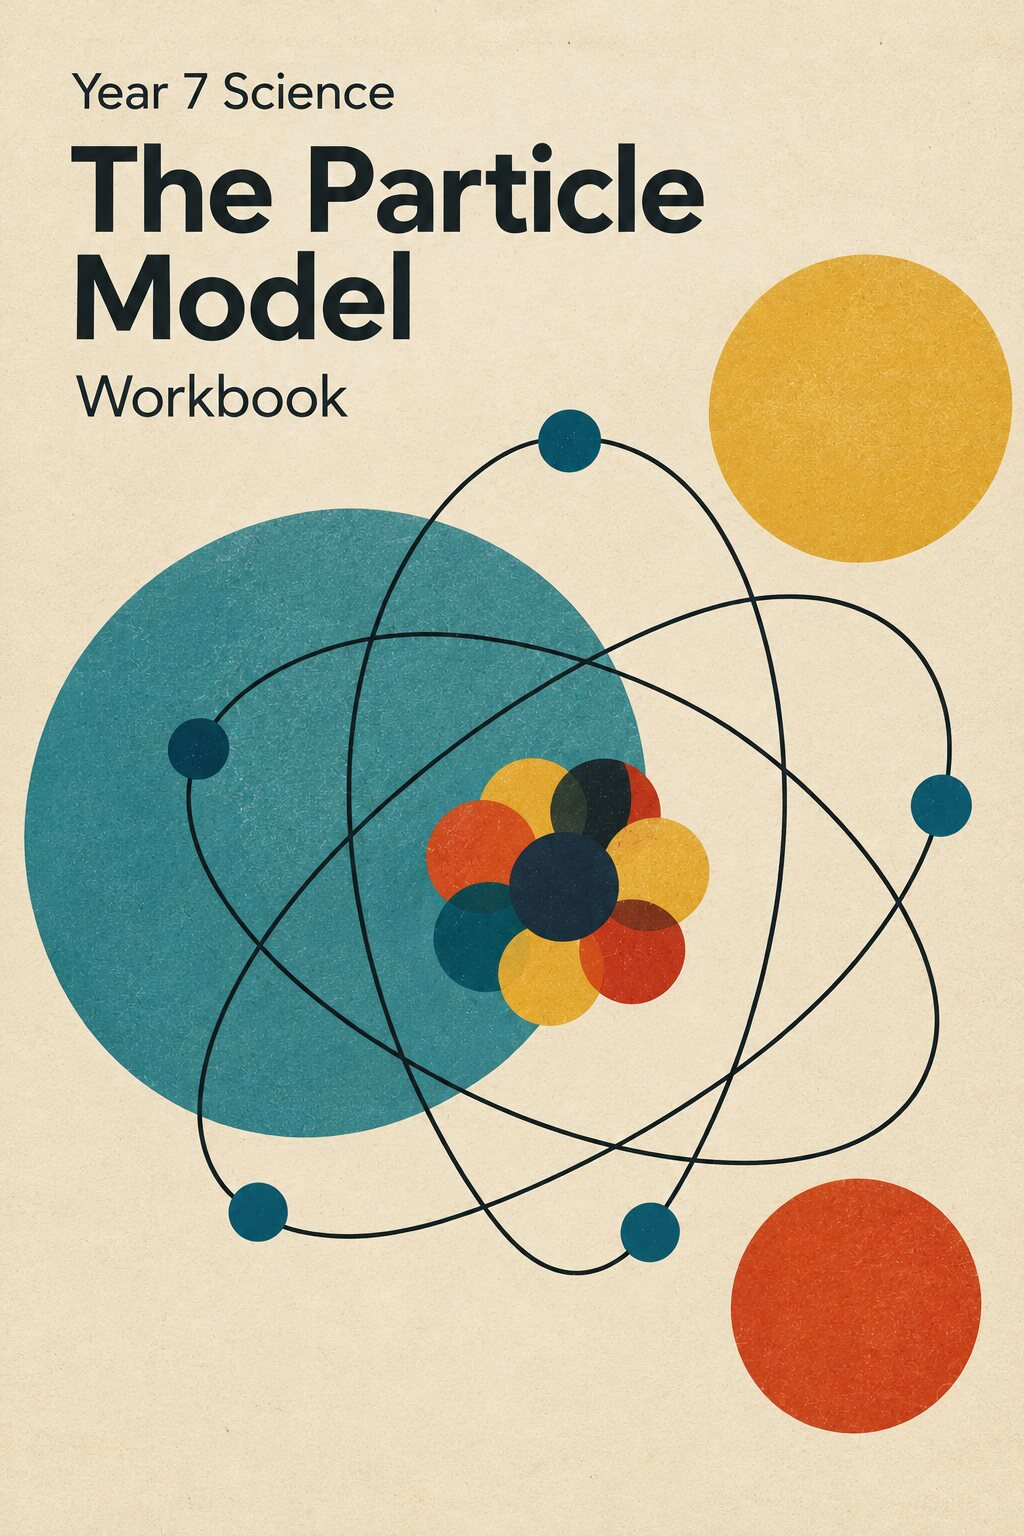
\includegraphics[width=\paperwidth]{../../../covers/particle-model.jpg}};
  \node[anchor=north east, fill=white, draw=Ink, line width=0.6pt, rounded corners=1.2mm,
        inner xsep=2mm, inner ysep=1.8mm, text width=30mm, font=\headingfont\footnotesize]
    at ([xshift=-4mm, yshift=-4mm]current page.north east)
    {\textbf{Name}\par\vspace{4mm}\hrule\vspace{2mm}\textbf{Class}\par\vspace{4mm}\hrule};
  \node[anchor=south east, fill=white, draw=Ink, line width=0.6pt, rounded corners=1.2mm,
        inner xsep=2.6mm, inner ysep=2mm, font=\headingfont\bfseries, align=right]
    at ([xshift=-4mm, yshift=6mm]current page.south east)
    {Lesson Booklet 2\\[-1pt]{\normalfont\headingfont\scriptsize Lessons 5--8}};
\end{tikzpicture}
\mbox{}
\clearpage

% ---- Inside cover ---------------------------------------------------------
\thispagestyle{plain}
{\headingfont\bfseries\fontsize{22}{26}\selectfont The Particle Model}\par\vspace{1mm}
{\headingfont\large Lesson Booklet 2 \textbullet\ Lessons 5--8 \textbullet\ Year 7}\par\vspace{1mm}
{\small\itshape VC 2.0: VC2S8U05 \textbullet\ VC2S8I01--I08 \textbullet\ VC2S8H01}\par\vspace{4mm}
\textbf{Teacher}\ \hrulefill\par

\begin{countrybox}{Acknowledgement of Country}
This booklet was created on the unceded Country of the Wurundjeri Woi-wurrung people of the Kulin Nation. We acknowledge Elders past, present and emerging.
\end{countrybox}

\begin{infobox}{How this booklet works}
One section for each lesson. Each opens with its key vocabulary, then:\par\smallskip
\renewcommand{\arraystretch}{1.25}
\begin{tabular}{@{}p{24mm}p{70mm}@{}}
\textbf{Part A} & a reading with comprehension questions \\
\textbf{Part B} & the ideas, worked through \\
\textbf{Part C} & practice on your own \\
\textbf{Part D} & above level: Year 8 extension \\
\end{tabular}

\smallskip
\begin{tabular}{@{}p{24mm}p{70mm}@{}}
\textbf{I do} \tagicon{\icodots{1}} & your teacher works an example (solid frame) \\
\textbf{We do} \tagicon{\icodots{2}} & you try one together (dashed frame) \\
\textbf{Reading} \tagicon{\icoread} & a passage to read (thin frame) \\
\textbf{Above level} \tagicon{\icoup} & extension (double frame) \\
\end{tabular}

\smallskip
Two lesson books; experiments are in the \textbf{Experiment Booklet}.
\end{infobox}

\clearpage
\markboth{Contents}{Contents}
{\headingfont\bfseries\LARGE Contents}\par\vspace{1mm}\noindent\rule{\linewidth}{0.6pt}\par\vspace{2mm}
\renewcommand{\arraystretch}{1.45}
\begin{tabular}{|C{1.1cm}|L{6.0cm}|C{2.4cm}|}
  \hline\thead{Lesson} & \thead{Title} & \thead{Page} \\ \hline
  1 & States of Matter & Book 1 \\ \hline
  2 & What is a Scientific Model? & Book 1 \\ \hline
  3 & \textit{Experiment 1 --- Matter Has Mass and Takes Up Space} & Experiment Booklet \\ \hline
  4 & The Particle Model & Book 1 \\ \hline
  5 & \hyperlink{lesson.5.1}{Changes of State} & \hyperlink{lesson.5.1}{p.\ \pageref{sec:7}} \\ \hline
  6 & \textit{Experiment 2 --- A Cooling Curve} & Experiment Booklet \\ \hline
  7 & \hyperlink{lesson.7.1}{Expansion, Contraction and Diffusion} & \hyperlink{lesson.7.1}{p.\ \pageref{sec:10}} \\ \hline
  8 & \hyperlink{lesson.8.1}{Density} & \hyperlink{lesson.8.1}{p.\ \pageref{sec:13}} \\ \hline
  9 & \textit{Experiment 3 --- Density by Displacement} & Experiment Booklet \\ \hline
  --- & \hyperlink{glossary}{Glossary} & \hyperlink{glossary}{\pageref{sec:glossary}} \\ \hline
\end{tabular}
\renewcommand{\arraystretch}{1}
\clearpage
\setcounter{section}{4}\renewcommand{\lessonart}{7}
% ══════════════════════════════════════════════════════════════════════════════
%  LESSON 7 — MELTING AND FREEZING                                  (Week 3 · P1)
% ══════════════════════════════════════════════════════════════════════════════
\sectiondiv{Changes of State}{Changes of state \textbullet{} Melting point \textbullet{} Evaporation and boiling compared \textbullet{} Boiling point}\label{sec:7}
\lessoncodes{VC2S8U05 \textbullet{} VC2S8I04}

\vocabhead
\begin{ctab}
\begin{tabular}{|SW{2.91cm}|W{8.05cm}|}
  \hd & \thead{Word} & \thead{Definition (copy from the slide)} \\ \hline
  & \scaf{\textbf{Change of state}\label{voc:change-of-state}} & \scaf{When a substance changes from one state to another, such as from solid to liquid.} \\ \hline
  & \textbf{Melting}\label{voc:melting} & \\ \hline
  & \textbf{Freezing}\label{voc:freezing} & \\ \hline
  & \textbf{Melting point}\label{voc:melting-point} & \\ \hline
  & \textbf{Physical change}\label{voc:physical-change} & \\ \hline
  & \textbf{Heating curve}\label{voc:heating-curve} & \\ \hline
  & \textbf{Evaporation}\label{voc:evaporation} & \\ \hline
  & \textbf{Boiling}\label{voc:boiling} & \\ \hline
  & \textbf{Boiling point}\label{voc:boiling-point} & \\ \hline
  & \textbf{Condensation}\label{voc:condensation} & \\ \hline
  & \textbf{Water vapour}\label{voc:water-vapour} & \\ \hline
  & \textbf{Sublimation}\label{voc:sublimation} & \\ \hline
\end{tabular}
\end{ctab}

% ─── PART A ───────────────────────────────────────────────────────────────────
\lessonpart{A}{Reading and comprehension}{Teal}\label{read:7}

\begin{readingbox}{Reading --- Ice That Won't Warm Up}
Put a thermometer into a glass of crushed ice and stir. The reading drops to about 0\,\textdegree C and stays there. Leave the glass on a sunny windowsill and the ice starts to turn into water --- but the thermometer still reads 0\,\textdegree C. For as long as there is ice in the glass, the temperature hardly changes, even though the sun is pouring energy into it. Only when the last piece of ice has gone does the water start to warm up.

Turning ice into water is a \textbf{change of state}. Changing from a solid to a liquid is called \textbf{melting}, and changing from a liquid to a solid is called \textbf{freezing}. Each pure substance melts at its own temperature, called its \textbf{melting point}. For water it is 0\,\textdegree C; for chocolate it is about 34\,\textdegree C, just below body temperature, which is why it melts in your mouth; for iron it is about 1540\,\textdegree C.

Melting is a \textbf{physical change}. No new substance is made: the water from melted ice can be frozen back into ice, and it is still the same water. Its particles are the same particles. Only the way they are arranged, and how they move, has changed.

So where does the sun's energy go while the ice is melting? It is used to pull the particles free from the fixed places that hold them in the solid. That is why the temperature stays flat. Scientists show this on a \textbf{heating curve}, a graph of temperature against time, where melting appears as a flat line.
\end{readingbox}

\rcreset
\rcq{What temperature does the thermometer show while the ice is melting?}{1.4cm}
\rcq{What is a change of state? Give the passage's example.}{1.8cm}
\rcq{What is the difference between melting and freezing?}{1.6cm}
\rcq{Why does chocolate melt in your mouth? Use a number from the passage.}{1.8cm}
\rcq{Explain why melting is a physical change.}{1.8cm}
\rcq{What happens to the particles of ice when it melts?}{1.8cm}
\rcq{Where does the sun's energy go while the ice is melting?}{1.8cm}
\rcq{How does melting show up on a heating curve?}{1.6cm}

% ─── PART B ───────────────────────────────────────────────────────────────────
\lessonpart{B}{Theory and examples}{Blue}\label{theory:7}

\subsection{The Changes of State}\label{sub:7.1}

\begin{center}
\begin{fitbox}\begin{tikzpicture}[font=\small, every node/.style={align=center}]
  \node[draw=NavyBlue, fill=LightBlue, rounded corners, minimum width=2.6cm, minimum height=1cm, font=\bfseries] (s) at (0,0) {SOLID};
  \node[draw=NavyBlue, fill=LightBlue, rounded corners, minimum width=2.6cm, minimum height=1cm, font=\bfseries] (l) at (5.5,0) {LIQUID};
  \node[draw=NavyBlue, fill=LightBlue, rounded corners, minimum width=2.6cm, minimum height=1cm, font=\bfseries] (g) at (11,0) {GAS};
  \draw[thin arrow, OrangeDark] ([yshift=4pt]s.east) -- node[above] {melting} ([yshift=4pt]l.west);
  \draw[thin arrow, MidBlue] ([yshift=-4pt]l.west) -- node[below] {freezing} ([yshift=-4pt]s.east);
  \draw[thin arrow, OrangeDark] ([yshift=4pt]l.east) -- node[above] {boiling or\\evaporation} ([yshift=4pt]g.west);
  \draw[thin arrow, MidBlue] ([yshift=-4pt]g.west) -- node[below] {condensation} ([yshift=-4pt]l.east);
  \draw[thin arrow, OrangeDark] (s.north) to[bend left=20] node[above] {sublimation} (g.north);
  \draw[thin arrow, MidBlue] (g.south) to[bend left=20] node[below] {deposition} (s.south);
  \node[font=\scriptsize, text=OrangeDark] at (-1.8,1.6) {\textbf{red:} energy in (heating)};
  \node[font=\scriptsize, text=MidBlue] at (-1.8,-1.6) {\textbf{blue:} energy out (cooling)};
\end{tikzpicture}\end{fitbox}
\end{center}
\figcap{The six changes of state. Melting and freezing come first; the rest follow.}

\subsection{Melting and Freezing With Particles}\label{sub:7.2}

\begin{workedex}{Explaining melting}
Explain, using particles, what happens when a block of butter melts in a hot pan.

\medskip
The pan heats the butter, so its particles gain energy and \textbf{vibrate faster}. At the melting point, they vibrate hard enough to \textbf{break free of their fixed places}. They stay close together but can now slide past each other, so the butter becomes a liquid.
\end{workedex}

\begin{wedo}{Explaining freezing}
Explain, using particles, what happens when water in an ice-cube tray freezes in the freezer.
\answerbox{3.2cm}
\end{wedo}

\subsection{Melting Point}\label{sub:7.3}

\begin{ctab}
\begin{tabular}{|L{5.0cm}|C{4.0cm}|}
  \thead{Substance} & \thead{Melting point (\textdegree C)} \\ \hline
  Oxygen & $-218$ \\ \hline
  Mercury & $-39$ \\ \hline
  Water & 0 \\ \hline
  Chocolate (about) & 34 \\ \hline
  Candle wax (about) & 60 \\ \hline
  Table salt & 801 \\ \hline
  Iron & 1538 \\ \hline
\end{tabular}
\end{ctab}

\begin{infobox}{Deciding a state from the melting point}
If the temperature is \textbf{below} a substance's melting point, it is a \textbf{solid}. If the temperature is \textbf{above} its melting point (and below its boiling point), it is a \textbf{liquid}.
\end{infobox}

\begin{workedex}{Which state?}
Mercury melts at $-39$\,\textdegree C. Is mercury a solid or a liquid in a classroom at 20\,\textdegree C?

\medskip
20\,\textdegree C is \textbf{above} the melting point of $-39$\,\textdegree C, so the mercury has already melted. \textbf{Mercury is a liquid at room temperature.}
\end{workedex}

\begin{wedo}{Which state?}
Candle wax melts at about 60\,\textdegree C.
\pt{a}Is candle wax a solid or a liquid on a 35\,\textdegree C day? Explain.
\answerbox{1.8cm}
\pt{b}Next to a candle flame the wax reaches 80\,\textdegree C. What state is it in there?
\answerbox{1.4cm}
\end{wedo}

\subsection{Reading a Heating Curve}\label{sub:7.4}

\diagHeatingCurve{1}
\figcap{Heating curve for ice, starting at $-20$\,\textdegree C. The flat parts are changes of state.}

\begin{workedex}{Reading a heating curve}
Use the heating curve above to answer: how long did the ice take to melt, and what was the temperature while it melted?

\medskip
The \textbf{first flat part} is melting. It starts at 1 minute and ends at 3 minutes, so melting took \textbf{2 minutes}. The temperature stayed at \textbf{0\,\textdegree C}, the melting point of water.
\end{workedex}

\needspace{20\baselineskip}
\begin{wedo}{Reading a heating curve}
A heating curve for water shows a flat part at 100\,\textdegree C from 6 minutes to 10 minutes.
\pt{a}What change of state is happening during this flat part?
\answerbox{1.4cm}
\pt{b}How long does it take?
\answerbox{1.4cm}
\pt{c}Why does the temperature not rise during this time?
\answerbox{2.2cm}
\end{wedo}

% ─── PART C ───────────────────────────────────────────────────────────────────

\subsection{Evaporation and Boiling Compared}\label{sub:8.1}

\begin{ctab}
\begin{tabular}{|L{2.56cm}|L{3.99cm}|L{3.99cm}|}
  \thead{} & \thead{Evaporation} & \thead{Boiling} \\ \hline
  Temperature & any temperature & only at the boiling point \\ \hline
  Where & only at the surface & all through the liquid (bubbles) \\ \hline
  Speed & slow & fast \\ \hline
  Particles & only the fastest surface particles escape & particles everywhere have enough energy to escape \\ \hline
\end{tabular}
\end{ctab}

\begin{workedex}{Why washing dries faster on a warm, windy day}
Explain, using particles, why wet clothes on a line dry faster on a warm, windy day than on a cold, still day.

\medskip
\textbf{Warm:} the water particles have more kinetic energy, so more of them are moving fast enough to escape from the surface.

\textbf{Windy:} the wind carries away the water vapour near the clothes, so escaped particles are less likely to bump back into the cloth.

\medskip
So more particles leave each second, and the clothes dry faster.
\end{workedex}

\begin{wedo}{Why a puddle dries faster when it is spread out}
Two puddles hold the same amount of water. One is deep and narrow; the other is shallow and spread out. Explain, using particles, which one evaporates first.
\answerbox{3.0cm}
\end{wedo}

\subsection{Boiling Point}\label{sub:8.2}

\begin{ctab}
\begin{tabular}{|L{4.11cm}|C{3.22cm}|C{3.22cm}|}
  \thead{Substance} & \thead{Melting point (\textdegree C)} & \thead{Boiling point (\textdegree C)} \\ \hline
  Oxygen & $-218$ & $-183$ \\ \hline
  Ethanol (alcohol) & $-114$ & 78 \\ \hline
  Water & 0 & 100 \\ \hline
  Mercury & $-39$ & 357 \\ \hline
  Iron & 1538 & 2862 \\ \hline
\end{tabular}
\end{ctab}

\begin{infobox}{Which state? Use both numbers}
Below the melting point: \textbf{solid}. Between the melting point and the boiling point: \textbf{liquid}. Above the boiling point: \textbf{gas}.
\end{infobox}

\begin{workedex}{Which state?}
Ethanol melts at $-114$\,\textdegree C and boils at 78\,\textdegree C. What state is it in at 90\,\textdegree C?

\medskip
90\,\textdegree C is \textbf{above} the boiling point of 78\,\textdegree C. \textbf{Ethanol is a gas at 90\,\textdegree C.}
\end{workedex}

\begin{wedo}{Which state?}
Oxygen melts at $-218$\,\textdegree C and boils at $-183$\,\textdegree C. What state is oxygen in at each temperature?
\pt{a}At $-200$\,\textdegree C.
\answerbox{1.4cm}
\pt{b}At room temperature, 20\,\textdegree C.
\answerbox{1.4cm}
\end{wedo}

\subsection{Condensation and Sublimation}\label{sub:8.3}

\begin{workedex}{Explaining condensation}
A cold can of drink is taken out of the fridge. Within a minute its outside is covered in drops of water. Explain, using particles.

\medskip
Air contains water vapour particles, moving fast. When they hit the cold can, they \textbf{lose energy} and slow down. Their attraction pulls them close together, and they \textbf{condense} into drops of liquid water on the can.
\end{workedex}

\begin{wedo}{Explaining condensation}
After a hot shower, the bathroom mirror is covered in fog. Explain, using particles, where the water comes from and why it forms on the mirror.
\answerbox{3.0cm}
\end{wedo}

% ─── PART C ───────────────────────────────────────────────────────────────────
\lessonpart{C}{Practice}{Amber}\label{prac:7}

Work through every task. Use the melting points in each question.

\needspace{12\baselineskip}
\task Name each change of state.

\vspace{4pt}
\begin{ctab}
\begin{tabular}{|SW{3.78cm}|Z{1.28cm}|W{3.78cm}|Z{1.28cm}|}
  \hd & \thead{Event} & \thead{Change} & \thead{Event} & \thead{Change} \\ \hline
  & An ice block melts in the sun & \scaf{melting} & Lava cools into rock & \scaf{freezing} \\ \hline
  & Wax drips and hardens & & Butter softens into a puddle & \\ \hline
  & A pond ices over & & An ice-cream drips & \\ \hline
\end{tabular}
\end{ctab}

\needspace{14\baselineskip}
\task Use the melting points to decide whether each substance is a solid or a liquid at 25\,\textdegree C.

\vspace{4pt}
\begin{ctab}
\begin{tabular}{|SW{3.85cm}|Z{3.35cm}|Z{3.35cm}|}
  \hd & \thead{Substance} & \thead{Melting point (\textdegree C)} & \thead{Solid or liquid at 25\,\textdegree C?} \\ \hline
  & \scaf{Iron} & \scaf{1538} & \scaf{solid} \\ \hline
  & Olive oil & $-6$ & \\ \hline
  & Coconut oil & 24 & \\ \hline
  & Table salt & 801 & \\ \hline
\end{tabular}
\end{ctab}

\taskpair{Explain why melting is a physical change.}{2.4cm}
         {Explain why chocolate melts in your hand but not in the pantry.}{2.4cm}

\needspace{12\baselineskip}
\task Name the change of state.

\vspace{4pt}
\begin{ctab}
\begin{tabular}{|SW{3.60cm}|Z{1.60cm}|W{3.33cm}|Z{1.60cm}|}
  \hd & \thead{Event} & \thead{Change} & \thead{Event} & \thead{Change} \\ \hline
  & A kettle bubbles & \scaf{boiling} & Breath fogs a cold window & \scaf{condensation} \\ \hline
  & A wet towel dries & & Dew forms on grass at night & \\ \hline
  & Dry ice shrinks without melting & & Frost forms on a car & \\ \hline
\end{tabular}
\end{ctab}

\needspace{14\baselineskip}
\task Use the melting and boiling points to name the state of each substance at 20\,\textdegree C.

\vspace{4pt}
\begin{ctab}
\begin{tabular}{|SW{2.60cm}|Z{2.46cm}|Z{2.46cm}|Z{2.60cm}|}
  \hd & \thead{Substance} & \thead{Melting point (\textdegree C)} & \thead{Boiling point (\textdegree C)} & \thead{State at 20\,\textdegree C} \\ \hline
  & \scaf{Water} & \scaf{0} & \scaf{100} & \scaf{liquid} \\ \hline
  & Nitrogen & $-210$ & $-196$ & \\ \hline
  & Sulfur & 115 & 445 & \\ \hline
  & Ethanol & $-114$ & 78 & \\ \hline
\end{tabular}
\end{ctab}

\taskpair{Give two ways that evaporation is different from boiling.}{2.6cm}
         {Explain why a bubble forms inside boiling water. What is inside the bubble?}{2.6cm}

\lessonpart{D}{Above level}{Violet}\label{ext:7}

\begin{yr8box}
These questions go beyond the Year 7 standard. They ask you to reason about energy and interpret data.

\medskip
\begin{keepext}
\needspace{10\baselineskip}
\exttask Salt is spread on icy roads in cold countries. Salty water can stay liquid down to about $-10$\,\textdegree C, instead of freezing at 0\,\textdegree C. Explain why this makes the roads safer on a $-5$\,\textdegree C morning.
\answerbox{2.8cm}
\end{keepext}

\begin{keepext}
\needspace{10\baselineskip}
\exttask A pure substance has a sharp melting point. A mixture, like chocolate or candle wax, melts gradually over a range of temperatures. Suggest how you could use a melting point test to check whether a sample of a white powder is pure.
\answerbox{3.0cm}
\end{keepext}

\end{yr8box}
\newpage
\setcounter{section}{6}\renewcommand{\lessonart}{10}
% ══════════════════════════════════════════════════════════════════════════════
%  LESSON 10 — DIFFUSION                                            (Week 4 · P1)
% ══════════════════════════════════════════════════════════════════════════════
\sectiondiv{Expansion, Contraction and Diffusion}{Particles spreading out \textbullet{} Diffusion in liquids and gases \textbullet{} Why things get bigger when heated \textbullet{} Expansion in solids, liquids and gases}\label{sec:10}
\lessoncodes{VC2S8U05 \textbullet{} VC2S8I01 \textbullet{} VC2S8I03 \textbullet{} VC2S8I06}

\vocabhead
\begin{ctab}
\begin{tabular}{|SW{2.91cm}|W{8.05cm}|}
  \hd & \thead{Word} & \thead{Definition (copy from the slide)} \\ \hline
  & \scaf{\textbf{Diffusion}\label{voc:diffusion}} & \scaf{Particles spreading out on their own from where there are many to where there are few.} \\ \hline
  & \textbf{Concentration}\label{voc:concentration} & \\ \hline
  & \textbf{Spread}\label{voc:spread} & \\ \hline
  & \textbf{Rate}\label{voc:rate} & \\ \hline
  & \textbf{Variable}\label{voc:variable} & \\ \hline
  & \textbf{Fair test}\label{voc:fair-test} & \\ \hline
  & \textbf{Expansion}\label{voc:expansion} & \\ \hline
  & \textbf{Contraction}\label{voc:contraction} & \\ \hline
  & \textbf{Expansion gap}\label{voc:expansion-gap} & \\ \hline
  & \textbf{Thermometer}\label{voc:thermometer} & \\ \hline
  & \textbf{Engineer}\label{voc:engineer} & \\ \hline
  & \textbf{Bimetallic strip}\label{voc:bimetallic-strip} & \\ \hline
\end{tabular}
\end{ctab}

% ─── PART A ───────────────────────────────────────────────------------------------
\lessonpart{A}{Reading and comprehension}{Teal}\label{read:10}

\begin{readingbox}{Reading --- The Uninvited Smell}
Somebody in the kitchen burns the toast. Within a minute everyone in the house knows about it, even with the doors shut. Nobody blew the smell through the house. It \textbf{spread} on its own, carried by the endless random movement of particles. This is \textbf{diffusion}: particles moving from a place where there are lots of them to places where there are few, until they are evenly mixed.

Scientists describe how crowded a substance is with the word \textbf{concentration}. Right next to the toaster, the concentration of smoke particles is high. In the bedroom, it starts at zero. Particles are always moving in random directions, so more of them wander out of the crowded area than wander into it. Over time, the concentration evens out.

Diffusion happens in liquids too. Drop food colouring into a still glass of water and watch: a coloured cloud slowly spreads until the whole glass is the same colour, without any stirring. It is much slower than in a gas, because liquid particles are packed closely together and keep bumping into one another. In solids, where particles are held in place, diffusion hardly happens at all.

The \textbf{rate} of diffusion means how fast it happens. Because particles move faster when they are hotter, you might predict that diffusion is faster in hot water. In today's prac you will test that prediction. To make it a \textbf{fair test}, you will change only one \textbf{variable} --- the temperature of the water --- and keep everything else the same.
\end{readingbox}

\rcreset
\rcq{How does the smell of burnt toast reach a bedroom with the door shut?}{1.8cm}
\rcq{Use the passage to write a definition of diffusion.}{1.8cm}
\rcq{What does concentration mean? Where is the concentration of smoke particles highest?}{1.8cm}
\rcq{Why do more particles move out of a crowded area than into it?}{1.8cm}
\rcq{Why is diffusion slower in a liquid than in a gas?}{1.6cm}
\rcq{Why does diffusion hardly happen in a solid?}{1.6cm}
\rcq{What is the rate of diffusion?}{1.4cm}
\rcq{In today's prac, which variable will you change, and why must everything else stay the same?}{1.8cm}

% ─── PART B ───────────────────────────────────────────────────────────────────
\lessonpart{B}{Theory and examples}{Blue}\label{theory:10}

\subsection{Diffusion With Particles}\label{sub:10.1}

\begin{center}\begin{fitbox}\begin{tikzpicture}[font=\small]
  \begin{scope}
    \foreach \x/\y in {0.3/0.3,0.65/0.3,1.0/0.3,1.35/0.3,1.7/0.3,2.05/0.3,2.35/0.3,0.3/0.65,0.7/0.66,1.1/0.64,1.5/0.66,1.9/0.65,2.3/0.64,0.35/1.0,0.75/1.02,1.15/1.0,1.55/1.0,1.95/1.02,2.3/1.0,0.3/1.38,0.7/1.36,1.1/1.38,1.5/1.36,1.9/1.38,2.3/1.36,0.35/1.73,0.75/1.75,1.15/1.73,1.55/1.75,1.95/1.73,2.3/1.75}{\node[pA, minimum size=2.6mm] at (\x,\y) {};}
    \foreach \x/\y in {1.0/1.92,1.3/2.15,1.6/1.92,1.15/2.4,1.45/2.42}{\node[pB, minimum size=2.6mm] at (\x,\y) {};}
    \draw[boxline] (0,0) rectangle (2.6,2.7);
    \node[font=\small\bfseries, text=NavyBlue] at (1.3,-0.35) {just added};
  \end{scope}
  \draw[thin arrow, DarkGrey] (3.0,1.3) -- (3.8,1.3);
  \begin{scope}[xshift=4.2cm]
    \foreach \x/\y in {0.3/0.3,0.65/0.3,1.0/0.3,1.35/0.3,1.7/0.3,2.05/0.3,2.35/0.3,0.3/0.65,0.7/0.66,1.1/0.64,1.5/0.66,1.9/0.65,2.3/0.64,0.35/1.0,0.75/1.02,1.15/1.0,1.55/1.0,1.95/1.02,2.3/1.0,0.3/1.38,0.7/1.36,1.1/1.38,1.5/1.36,1.9/1.38,2.3/1.36,0.35/1.73,0.75/1.75,1.15/1.73,1.55/1.75,1.95/1.73,2.3/1.75,1.3/2.12,0.7/2.1,1.9/2.1}{\node[pA, minimum size=2.6mm] at (\x,\y) {};}
    \foreach \x/\y in {0.3/2.1,2.3/2.12,1.1/0.82,0.5/1.55,2.1/0.47}{\node[pB, minimum size=2.6mm] at (\x,\y) {};}
    \draw[boxline] (0,0) rectangle (2.6,2.7);
    \node[font=\small\bfseries, text=NavyBlue] at (1.3,-0.35) {later: evenly spread};
  \end{scope}
  \node[pB, minimum size=2.6mm] at (8.2,1.6) {}; \node[anchor=west, lab, font=\small] at (8.4,1.6) {food colouring};
  \node[pA, minimum size=2.6mm] at (8.2,1.0) {}; \node[anchor=west, lab, font=\small] at (8.4,1.0) {water};
\end{tikzpicture}\end{fitbox}\end{center}
\figcap{Diffusion of food colouring in water. Nothing stirs it: the random movement of the particles mixes them.}

\begin{workedex}{Explaining diffusion}
A teabag is put into a cup of still hot water. A brown colour slowly spreads through the whole cup. Explain, using particles.

\medskip
The tea particles start at a \textbf{high concentration} near the teabag. The tea and water particles are always \textbf{moving in random directions} and bumping into each other, so the tea particles gradually spread out to where there are fewer of them, until they are \textbf{evenly mixed}.
\end{workedex}

\begin{wedo}{Explaining diffusion}
An air freshener is sprayed in one corner of a room. Explain, using particles, how the smell reaches the other side.
\answerbox{3.0cm}
\end{wedo}

\subsection{Prac: Food Colouring in Hot and Cold Water}\label{sub:10.2}

\begin{scaffold}{Prediction}
Will the food colouring spread faster in hot water or in cold water? Give a particle reason.
\answerbox{2cm}
\end{scaffold}

\subsubsection*{Equipment}
Two identical 250\,mL beakers \quad 200\,mL cold tap water \quad 200\,mL hot water from the kettle (teacher pours) \quad Food colouring with a dropper \quad Stopwatch \quad White sheet of paper

\subsubsection*{Method}
\begin{enumerate}[itemsep=2pt]
  \item Stand both beakers on white paper. Put 200\,mL of cold water in one and 200\,mL of hot water in the other. Let them stand for a minute so the water is still.
  \item At the same moment, gently add \textbf{one} drop of food colouring to the middle of each beaker. Do not stir or bump the beakers.
  \item Start the stopwatch. Record what you see after 1, 3 and 5 minutes.
  \item Record the time when each beaker looks evenly coloured.
\end{enumerate}

\begin{infobox}{Safety}
Hot water can scald. Only your teacher pours hot water. Do not move the beaker of hot water, and keep it away from the edge of the bench.
\end{infobox}

\needspace{14\baselineskip}
\begin{ctab}
\begin{tabular}{|SW{2.05cm}|W{4.24cm}|W{4.24cm}|}
  \hd & \thead{Time} & \thead{Cold water} & \thead{Hot water} \\ \hline
  & \scaf{1 minute} & \scaf{a small cloud near the middle} & \scaf{a bigger cloud, spreading downwards} \\ \hline
  & 3 minutes & & \\ \hline
  & 5 minutes & & \\ \hline
  & Evenly coloured at & & \\ \hline
\end{tabular}
\end{ctab}

\subsection{Temperature and the Rate of Diffusion}\label{sub:10.3}

\begin{workedex}{Explaining the result}
In a prac, food colouring spread through hot water in 2 minutes but took 15 minutes in cold water. Explain the result using particles.

\medskip
In hot water the water particles have more \textbf{kinetic energy} and move faster. They knock the food colouring particles about harder and more often, so the colouring spreads out \textbf{faster}. The rate of diffusion is higher at a higher temperature.
\end{workedex}

\begin{wedo}{Fair testing}
In your prac, name the variable you changed, the one you observed, and two that you kept the same.
\pt{a}Changed.
\answerbox{1.4cm}
\pt{b}Observed.
\answerbox{1.4cm}
\pt{c}Kept the same.
\answerbox{1.6cm}
\end{wedo}

% ─── PART C ───────────────────────────────────────────────────────────────────

\subsection{Expansion With Particles}\label{sub:11.1}

\begin{center}\begin{fitbox}\begin{tikzpicture}[font=\small]
  \begin{scope}
    \foreach \r in {0,...,3}{\foreach \c in {0,...,5}{\node[pA, minimum size=3mm] at (0.25+\c*0.32,0.25+\r*0.32) {};}}
    \draw[DarkGrey, line width=0.8pt] (0.07,0.07) rectangle (1.93,1.43);
    \node[font=\small\bfseries, text=NavyBlue] at (1.0,-0.3) {cold};
  \end{scope}
  \draw[thin arrow, OrangeDark] (2.4,0.75) -- node[above, font=\scriptsize] {heat} (3.4,0.75);
  \begin{scope}[xshift=3.8cm]
    \foreach \r in {0,...,3}{\foreach \c in {0,...,5}{\node[pA, minimum size=3mm] at (0.25+\c*0.4,0.25+\r*0.4) {};}}
    \draw[DarkGrey, line width=0.8pt] (0.07,0.07) rectangle (2.43,1.68);
    \node[font=\small\bfseries, text=NavyBlue] at (1.25,-0.3) {hot: same particles, further apart};
  \end{scope}
\end{tikzpicture}\end{fitbox}\end{center}
\figcap{When a solid is heated, its particles vibrate more and sit a little further apart. They do not grow. (The change is exaggerated here.)}

\begin{workedex}{Explaining expansion}
A metal jar lid is stuck. Running it under hot water makes it easier to open. Explain, using particles.

\medskip
The hot water heats the metal lid. Its particles \textbf{vibrate faster} and push \textbf{further apart}, so the lid \textbf{expands} and gets slightly bigger. It loosens its grip on the glass jar, so it turns more easily.
\end{workedex}

\begin{wedo}{Explaining contraction}
A steel ball fits through a steel ring at room temperature. After the ring is left in the freezer, the ball no longer fits through it. Explain, using particles, why the ring got smaller.
\answerbox{3.0cm}
\end{wedo}

\subsection{Solids, Liquids and Gases Compared}\label{sub:11.2}

All three states expand when heated, but by very different amounts. Gases expand most, because their particles are hardly attracted to each other at all.

\begin{ctab}
\begin{tabular}{|L{1.83cm}|L{3.65cm}|L{5.06cm}|}
  \thead{State} & \thead{How much it expands} & \thead{Example} \\ \hline
  Solid & a tiny amount & railway tracks lengthen on hot days \\ \hline
  Liquid & more than a solid & the liquid in a thermometer rises \\ \hline
  Gas & much more than a liquid & a balloon grows when moved into the sun \\ \hline
\end{tabular}
\end{ctab}

\begin{workedex}{Expansion in a liquid}
A thermometer reading rises from 20\,\textdegree C to 30\,\textdegree C when it is put in warm water. Explain why the liquid moves up the tube.

\medskip
The warm water heats the liquid in the bulb. Its particles move faster and spread further apart, so the liquid \textbf{expands}. The only place it can go is up the narrow tube, so the level rises.
\end{workedex}

\begin{wedo}{Expansion in a gas}
An empty plastic bottle with its lid on is left in a hot car and becomes firm and swollen. Explain, using particles.
\answerbox{3.0cm}
\end{wedo}

\subsection{Designing for Expansion}\label{sub:11.3}

\begin{workedex}{Why power lines sag}
Overhead power lines are hung loosely in summer, so they sag between the poles. Explain why they are not pulled tight.

\medskip
In winter the cold wires \textbf{contract} and get shorter. If they were tight in summer, the shrinking in winter could pull them so hard that they snap or pull the poles over. Hanging them loosely leaves room to contract.
\end{workedex}

\begin{wedo}{Why concrete has gaps}
Explain why a long concrete driveway is laid with thin gaps every few metres. Say what could happen without them.
\answerbox{3.0cm}
\end{wedo}

% ─── PART C ───────────────────────────────────────────────────────────────────
\lessonpart{C}{Practice}{Amber}\label{prac:10}

Work through every task. In each explanation, mention random movement and concentration.

\needspace{12\baselineskip}
\task Write \textbf{YES} if the example is diffusion and \textbf{NO} if it is not.

\vspace{4pt}
\begin{ctab}
\begin{tabular}{|SW{3.91cm}|Z{1.21cm}|W{3.78cm}|Z{1.21cm}|}
  \hd & \thead{Example} & \thead{Diffusion?} & \thead{Example} & \thead{Diffusion?} \\ \hline
  & A smell spreading through a room & \scaf{YES} & Stirring sugar into tea & \scaf{NO} \\ \hline
  & Ink spreading in still water & & Wind blowing smoke away & \\ \hline
  & A drop of cordial colouring a jug of still water & & Pouring milk into a glass & \\ \hline
\end{tabular}
\end{ctab}

\taskpair{Explain why diffusion is faster in a gas than in a liquid.}{2.6cm}
         {Explain why diffusion hardly happens in a solid.}{2.6cm}

\needspace{10\baselineskip}
\task Explain, using particles, why a smell from a bakery spreads faster on a hot day than on a cold day.
\answerbox{3.0cm}

\needspace{12\baselineskip}
\task Write \textbf{EXPANDS} or \textbf{CONTRACTS} for each.

\vspace{4pt}
\begin{ctab}
\begin{tabular}{|SW{3.46cm}|Z{1.60cm}|W{3.46cm}|Z{1.60cm}|}
  \hd & \thead{Event} & \thead{Expands or contracts?} & \thead{Event} & \thead{Expands or contracts?} \\ \hline
  & A steel bridge on a hot day & \scaf{EXPANDS} & A balloon in the freezer & \scaf{CONTRACTS} \\ \hline
  & Thermometer liquid in hot tea & & Railway tracks on a frosty night & \\ \hline
  & A metal lid under hot water & & Air in a tyre on a cold morning & \\ \hline
\end{tabular}
\end{ctab}

\taskpair{Explain why railway tracks are laid with small gaps between sections.}{2.8cm}
         {Put solids, liquids and gases in order from most to least expansion.}{2.8cm}

\needspace{10\baselineskip}
\task Explain, using particles, why a balloon left in the sun gets bigger.
\answerbox{3.0cm}

\lessonpart{D}{Above level}{Violet}\label{ext:10}

\begin{yr8box}
These questions go beyond the Year 7 standard. They ask you to explain diffusion in living things and design tests.

\medskip
\begin{keepext}
\needspace{10\baselineskip}
\exttask Oxygen moves from the air in your lungs into your blood by diffusion. The air in the lungs has a high concentration of oxygen; blood arriving at the lungs has a low concentration. Explain why breathing in fresh air keeps the oxygen moving into the blood.
\answerbox{3.2cm}
\end{keepext}

\begin{keepext}
\needspace{10\baselineskip}
\exttask Design a fair test to find out whether diffusion is faster in water or in cooking oil. Name what you would change, what you would measure and two things you would keep the same.
\answerbox{3.4cm}
\end{keepext}

\end{yr8box}
\newpage
\setcounter{section}{7}\renewcommand{\lessonart}{13}
% ══════════════════════════════════════════════════════════════════════════════
%  LESSON 13 — WHAT DENSITY MEANS                                   (Week 5 · P1)
% ══════════════════════════════════════════════════════════════════════════════
\sectiondiv{Density}{Heavy for its size \textbullet{} Density and particles \textbullet{} The density formula \textbullet{} Volume of a block}\label{sec:13}
\lessoncodes{VC2S8U05 \textbullet{} VC2S8I04}

\vocabhead
\begin{ctab}
\begin{tabular}{|SW{2.91cm}|W{8.05cm}|}
  \hd & \thead{Word} & \thead{Definition (copy from the slide)} \\ \hline
  & \scaf{\textbf{Density}\label{voc:density}} & \scaf{How much mass is packed into a certain volume of a substance.} \\ \hline
  & \textbf{Dense}\label{voc:dense} & \\ \hline
  & \textbf{Float}\label{voc:float} & \\ \hline
  & \textbf{Sink}\label{voc:sink} & \\ \hline
  & \textbf{Cubic centimetre (cm\textsuperscript{3})} & \\ \hline
  & \textbf{Compare}\label{voc:compare} & \\ \hline
  & \textbf{Formula}\label{voc:formula} & \\ \hline
  & \textbf{Mass ($m$)}\label{voc:mass-m} & \\ \hline
  & \textbf{Volume ($V$)}\label{voc:volume-v} & \\ \hline
  & \textbf{Density ($D$)}\label{voc:density-d} & \\ \hline
  & \textbf{g/cm\textsuperscript{3}} & \\ \hline
  & \textbf{Identify}\label{voc:identify} & \\ \hline
\end{tabular}
\end{ctab}

% ─── PART A ───────────────────────────────────────────────────────────────────
\lessonpart{A}{Reading and comprehension}{Teal}\label{read:13}

\begin{readingbox}{Reading --- Heavier Than It Looks}
Which is heavier: a kilogram of feathers or a kilogram of bricks? It is a trick question --- they both have a mass of one kilogram. But the feathers fill a huge bag, and the bricks fit in your hand. The bricks are much more \textbf{dense}. \textbf{Density} tells you how much mass is packed into a certain volume of a substance.

Scientists often compare densities using a small block one centimetre long on each side. Its volume is one \textbf{cubic centimetre}, written 1\,cm\textsuperscript{3} --- the same as one millilitre. A cubic centimetre of water has a mass of 1\,g. A cubic centimetre of cork has a mass of only about 0.24\,g, and a cubic centimetre of gold has a mass of about 19\,g. Gold is about 19 times as dense as water.

The particle model explains why. Some substances are made of heavier particles than others. Some have their particles packed more tightly. The heavier the particles, and the closer together they are, the more mass is squeezed into each cubic centimetre.

Density also decides whether something will \textbf{float} or \textbf{sink}. An object that is less dense than water floats; one that is more dense sinks. That is why a log floats while a small pebble sinks, even though the log is far heavier. To decide, you must \textbf{compare} densities, not masses.
\end{readingbox}

\rcreset
\rcq{Why is ``Which is heavier, a kilogram of feathers or a kilogram of bricks?'' a trick question?}{1.8cm}
\rcq{Use the passage to write a definition of density.}{1.6cm}
\rcq{What is a cubic centimetre, and what is it equal to?}{1.6cm}
\rcq{What is the mass of 1\,cm\textsuperscript{3} of water, of cork and of gold?}{1.8cm}
\rcq{Give two particle reasons why one substance can be denser than another.}{1.8cm}
\rcq{What decides whether an object floats or sinks in water?}{1.6cm}
\rcq{Why does a heavy log float when a light pebble sinks?}{1.8cm}
\rcq{Why must you compare densities rather than masses to predict floating?}{1.8cm}

% ─── PART B ───────────────────────────────────────────────────────────────────
\lessonpart{B}{Theory and examples}{Blue}\label{theory:13}

\subsection{Density and Particles}\label{sub:13.1}

\begin{center}\begin{fitbox}\begin{tikzpicture}[font=\small]
  \begin{scope}
    \foreach \x/\y in \gaspos{\node[pA] at (\x,\y) {};}\pbox
    \node[font=\small\bfseries, text=NavyBlue, align=center] at (1.3,-0.5) {few particles\\low density};
  \end{scope}
  \begin{scope}[xshift=4.2cm]
    \stateIn{solid}{pA}
    \node[font=\small\bfseries, text=NavyBlue, align=center] at (1.3,-0.5) {packed tightly\\higher density};
  \end{scope}
  \begin{scope}[xshift=8.4cm]
    \stateIn{solid}{pB}
    \foreach \r in {0,...,4}{\foreach \c in {0,...,6}{\fill[OrangeDark] (0.31+\c*0.33,0.2+\r*0.33) circle (0.5pt);}}
    \node[font=\small\bfseries, text=NavyBlue, align=center] at (1.3,-0.5) {packed tightly, heavier\\particles: highest density};
  \end{scope}
\end{tikzpicture}\end{fitbox}\end{center}
\figcap{Three boxes of the same volume. More particles, or heavier particles, means more mass in the same space.}

\begin{workedex}{Explaining density with particles}
A cube of aluminium and a cube of lead are exactly the same size. The lead cube has more than four times the mass. Suggest a particle reason.

\medskip
Both are metals, so both have particles \textbf{packed tightly}. The lead must have \textbf{heavier particles}, so the same volume holds much more mass. Lead is \textbf{denser} than aluminium.
\end{workedex}

\begin{wedo}{Explaining density with particles}
A balloon full of air and a balloon full of water are the same size. Explain, using particles, why the water balloon is much heavier.
\answerbox{3.0cm}
\end{wedo}

\subsection{Floating and Sinking}\label{sub:13.2}

\begin{ctab}
\begin{tabular}{|L{3.73cm}|C{3.41cm}|C{3.41cm}|}
  \thead{Substance} & \thead{Density (g/cm\textsuperscript{3})} & \thead{In water} \\ \hline
  Cork & 0.24 & floats \\ \hline
  Pine wood & 0.5 & floats \\ \hline
  Ice & 0.92 & floats \\ \hline
  Water & 1.00 & --- \\ \hline
  Honey & 1.4 & sinks \\ \hline
  Aluminium & 2.7 & sinks \\ \hline
  Iron & 7.9 & sinks \\ \hline
  Gold & 19.3 & sinks \\ \hline
\end{tabular}
\end{ctab}

\begin{infobox}{The floating rule}
Less dense than water (less than 1\,g/cm\textsuperscript{3}): it \textbf{floats}. More dense than water (more than 1\,g/cm\textsuperscript{3}): it \textbf{sinks}.
\end{infobox}

\begin{workedex}{Float or sink?}
Olive oil has a density of 0.92\,g/cm\textsuperscript{3}. Will a layer of olive oil float on water or sink below it?

\medskip
0.92 is \textbf{less than} 1.00, so olive oil is less dense than water. \textbf{It floats on top of the water.}
\end{workedex}

\begin{wedo}{Float or sink?}
A rubber ball has a density of 1.1\,g/cm\textsuperscript{3}, and a plastic bottle cap has a density of 0.9\,g/cm\textsuperscript{3}. Decide whether each floats or sinks in water, and give a reason.
\pt{a}The rubber ball.
\answerbox{1.6cm}
\pt{b}The bottle cap.
\answerbox{1.6cm}
\end{wedo}

\subsection{Density of the Three States}\label{sub:13.3}

For most substances, the solid is the most dense, the liquid a little less dense, and the gas far less dense, because the gas particles are so far apart.

\begin{workedex}{Density and state}
Explain why steam is far less dense than liquid water.

\medskip
The particles are the same water particles. In steam they are \textbf{far apart}, so a cubic centimetre of steam holds far fewer particles, and so far less mass, than a cubic centimetre of liquid water.
\end{workedex}

\begin{wedo}{Density and state}
Ice floats on water, so ice is less dense than liquid water. Use the floating rule and the particle model to suggest what this tells us about how the particles in ice are arranged compared with liquid water.
\answerbox{3.0cm}
\end{wedo}

% ─── PART C ───────────────────────────────────────────────────────────────────

\subsection{The Density Formula}\label{sub:14.1}

\begin{infobox}{Density}
\[ \text{density} = \frac{\text{mass}}{\text{volume}} \qquad\Rightarrow\qquad \boxed{D = \frac{m}{V}} \]
Mass in grams (g), volume in cubic centimetres (cm\textsuperscript{3}) or millilitres (mL), density in g/cm\textsuperscript{3}. Remember: 1\,mL = 1\,cm\textsuperscript{3}.
\end{infobox}

\begin{workedex}{Calculating density}
A stone has a mass of 54\,g and a volume of 20\,cm\textsuperscript{3}. Calculate its density.

\medskip
$D = \dfrac{m}{V} = \dfrac{54}{20} = \mathbf{2.7\ g/cm^3}$
\end{workedex}

\begin{wedo}{Calculating density}
A piece of wood has a mass of 30\,g and a volume of 50\,cm\textsuperscript{3}. Calculate its density.
\workbox{2.6cm}
\end{wedo}

\subsection{Volume of a Block}\label{sub:14.2}

For a rectangular block, multiply the three side lengths: \quad $V = \text{length} \times \text{width} \times \text{height}$.

\begin{workedex}{Density of a block}
A block is 5\,cm long, 2\,cm wide and 2\,cm high, and has a mass of 54\,g. Find its density.

\medskip
\textbf{Volume:} $V = 5 \times 2 \times 2 = 20\ \text{cm}^3$

\textbf{Density:} $D = \dfrac{m}{V} = \dfrac{54}{20} = \mathbf{2.7\ g/cm^3}$
\end{workedex}

\begin{wedo}{Density of a block}
A block of wax is 4\,cm long, 3\,cm wide and 2\,cm high, and has a mass of 21.6\,g. Find its density.
\workbox{3.2cm}
\end{wedo}

\subsection{Identifying a Substance}\label{sub:14.3}

\begin{ctab}
\begin{tabular}{|L{2.79cm}|C{2.27cm}||L{2.79cm}|C{2.27cm}|}
  \thead{Substance} & \thead{g/cm\textsuperscript{3}} & \thead{Substance} & \thead{g/cm\textsuperscript{3}} \\ \hline
  Pine wood & 0.5 & Aluminium & 2.7 \\ \hline
  Candle wax & 0.9 & Iron & 7.9 \\ \hline
  Water & 1.0 & Copper & 8.9 \\ \hline
  Glass & 2.5 & Gold & 19.3 \\ \hline
\end{tabular}
\end{ctab}

\begin{workedex}{Identifying a substance}
A shiny metal cube has a mass of 79\,g and a volume of 10\,cm\textsuperscript{3}. Use the table to identify the metal. Will it float in water?

\medskip
$D = \dfrac{m}{V} = \dfrac{79}{10} = 7.9\ \text{g/cm}^3$ \quad --- this matches \textbf{iron}.

7.9 is more than 1.0, so it is denser than water and \textbf{sinks}.
\end{workedex}

\begin{wedo}{Identifying a substance}
A metal bar has a mass of 89\,g and a volume of 10\,cm\textsuperscript{3}. The densities to choose from are aluminium 2.7, iron 7.9, copper 8.9 and gold 19.3\,g/cm\textsuperscript{3}.
\pt{a}Calculate its density.
\workbox{2.2cm}
\pt{b}Identify the metal.
\answerbox{1.4cm}
\end{wedo}

% ─── PART C ───────────────────────────────────────────────────────────────────
\lessonpart{C}{Practice}{Amber}\label{prac:13}

Work through every task. To predict floating, always compare with water: 1\,g/cm\textsuperscript{3}.

\needspace{14\baselineskip}
\task Decide whether each substance floats or sinks in water.

\vspace{4pt}
\begin{ctab}
\begin{tabular}{|SW{3.83cm}|Z{3.35cm}|Z{3.35cm}|}
  \hd & \thead{Substance} & \thead{Density (g/cm\textsuperscript{3})} & \thead{Floats or sinks?} \\ \hline
  & \scaf{Glass} & \scaf{2.5} & \scaf{sinks} \\ \hline
  & Candle wax & 0.9 & \\ \hline
  & Copper & 8.9 & \\ \hline
  & Balsa wood & 0.16 & \\ \hline
  & Sea water & 1.03 & \\ \hline
\end{tabular}
\end{ctab}

\taskpair{A tennis ball and a golf ball are about the same size. Which is denser? Explain.}{2.6cm}
         {Explain why a heavy log floats but a small pebble sinks.}{2.6cm}

\needspace{10\baselineskip}
\task Put these in order from least dense to most dense: iron (7.9\,g/cm\textsuperscript{3}), cork (0.24\,g/cm\textsuperscript{3}), water (1.0\,g/cm\textsuperscript{3}), gold (19.3\,g/cm\textsuperscript{3}), ice (0.92\,g/cm\textsuperscript{3}).
\answerbox{2.0cm}

\needspace{14\baselineskip}
\task Complete the table. The first row has been done for you.

\vspace{4pt}
\begin{ctab}
\begin{tabular}{|SW{2.36cm}|Z{1.94cm}|Z{2.22cm}|Z{3.60cm}|}
  \hd & \thead{Object} & \thead{Mass (g)} & \thead{Volume (cm\textsuperscript{3})} & \thead{Density (g/cm\textsuperscript{3})} \\ \hline
  & Stone & 75 & 30 & \scaf{$75 \div 30 = 2.5$} \\ \hline
  & Cork & 12 & 50 & \\ \hline
  & Brass key & 34 & 4 & \\ \hline
  & Milk & 103 & 100 & \\ \hline
\end{tabular}
\end{ctab}

\taskpair{A 10\,cm\textsuperscript{3} piece of plastic has a mass of 12\,g. Find its density.}{2.8cm}
         {200\,mL of oil has a mass of 184\,g. Find its density.}{2.8cm}

\needspace{10\baselineskip}
\task A block of wood is 10\,cm long, 5\,cm wide and 2\,cm high, and has a mass of 50\,g.
\pt{a}Find its volume.
\workbox{1.8cm}
\pt{b}Find its density.
\workbox{1.8cm}
\pt{c}Will it float in water? Explain.
\answerbox{1.6cm}

\lessonpart{D}{Above level}{Violet}\label{ext:13}

\begin{yr8box}
These questions go beyond the Year 7 standard. They ask you to apply density to ships, balloons and the sea.

\medskip
\begin{keepext}
\needspace{10\baselineskip}
\exttask Steel has a density of 7.9\,g/cm\textsuperscript{3}, yet huge steel ships float. A ship is mostly air inside. Explain how a steel ship can float, using the idea of the density of the whole ship.
\answerbox{3.2cm}
\end{keepext}

\begin{keepext}
\needspace{10\baselineskip}
\exttask A hot-air balloon rises when the air inside it is heated. Explain, using particles and density, why hot air rises through cold air.
\answerbox{3.2cm}
\end{keepext}

\end{yr8box}
\newpage
\clearpage\markboth{Glossary}{Glossary}\hypertarget{glossary}{}\pdfbookmark[1]{Glossary}{glossarybm}
{\headingfont\bfseries\LARGE Glossary}\label{sec:glossary}\par\vspace{1mm}\noindent\rule{\linewidth}{0.6pt}\par
{\small Every key word in this booklet and the page it is introduced on.}\par\smallskip
\renewcommand{\arraystretch}{1.3}
\begin{longtable}{|>{\RaggedRight}p{34mm}|p{9mm}|p{\dimexpr\linewidth-43mm-6\tabcolsep-4\arrayrulewidth-1pt\relax}|}
\hline \rule{0pt}{4mm}\headingfont\bfseries Word & \headingfont\bfseries Page & \headingfont\bfseries In my own words \\ \hline \endhead
  Bimetallic strip & \pageref{voc:bimetallic-strip} & \\ \hline
  Boiling & \pageref{voc:boiling} & \\ \hline
  Boiling point & \pageref{voc:boiling-point} & \\ \hline
  Change of state & \pageref{voc:change-of-state} & \\ \hline
  Compare & \pageref{voc:compare} & \\ \hline
  Concentration & \pageref{voc:concentration} & \\ \hline
  Condensation & \pageref{voc:condensation} & \\ \hline
  Contraction & \pageref{voc:contraction} & \\ \hline
  Dense & \pageref{voc:dense} & \\ \hline
  Density & \pageref{voc:density} & \\ \hline
  Density ($D$) & \pageref{voc:density-d} & \\ \hline
  Diffusion & \pageref{voc:diffusion} & \\ \hline
  Engineer & \pageref{voc:engineer} & \\ \hline
  Evaporation & \pageref{voc:evaporation} & \\ \hline
  Expansion & \pageref{voc:expansion} & \\ \hline
  Expansion gap & \pageref{voc:expansion-gap} & \\ \hline
  Fair test & \pageref{voc:fair-test} & \\ \hline
  Float & \pageref{voc:float} & \\ \hline
  Formula & \pageref{voc:formula} & \\ \hline
  Freezing & \pageref{voc:freezing} & \\ \hline
  Heating curve & \pageref{voc:heating-curve} & \\ \hline
  Identify & \pageref{voc:identify} & \\ \hline
  Mass ($m$) & \pageref{voc:mass-m} & \\ \hline
  Melting & \pageref{voc:melting} & \\ \hline
  Melting point & \pageref{voc:melting-point} & \\ \hline
  Physical change & \pageref{voc:physical-change} & \\ \hline
  Rate & \pageref{voc:rate} & \\ \hline
  Sink & \pageref{voc:sink} & \\ \hline
  Spread & \pageref{voc:spread} & \\ \hline
  Sublimation & \pageref{voc:sublimation} & \\ \hline
  Thermometer & \pageref{voc:thermometer} & \\ \hline
  Variable & \pageref{voc:variable} & \\ \hline
  Volume ($V$) & \pageref{voc:volume-v} & \\ \hline
  Water vapour & \pageref{voc:water-vapour} & \\ \hline
\end{longtable}
\padtofour
\end{document}
